\documentclass{beamer}

\usepackage[size=custom,width=16,height=9,scale=0.4]{beamerposter}
% \usepackage[size=custom, width=12.8, height=9.6, scale=0.4]{beamerposter}

\usepackage[T1]{fontenc}
\usepackage{tcolorbox}
\usepackage{graphicx}
\usepackage{lmodern}
\usepackage{tabularx}
\usepackage{tikz}
\usepackage{blindtext}
\usepackage{svg}
\usepackage{booktabs}
\usepackage[style = ieee]{biblatex}
\usepackage{blindtext}
\usepackage{setspace}
\usepackage{minted}
\usepackage{nicematrix}
\usepackage{framed}
\usepackage{colortbl}
\usepackage{multirow}
\usepackage{multicol}
\usepackage{subfiles}

\usetikzlibrary{calc}
\usetikzlibrary{intersections,decorations.markings}

\usetikzlibrary{positioning}
\usetikzlibrary{ext.topaths.arcthrough}

\usepackage{subtikzpicture}

\usemintedstyle{dracula}

\renewcommand{\tabularxcolumn}[1]{m{#1}}

\makeatletter
\tikzset{
  use path for main/.code={%
    \tikz@addmode{%
      \expandafter\pgfsyssoftpath@setcurrentpath\csname tikz@intersect@path@name@#1\endcsname
    }%
  },
  use path for actions/.code={%
    \expandafter\def\expandafter\tikz@preactions\expandafter{\tikz@preactions\expandafter\let\expandafter\tikz@actions@path\csname tikz@intersect@path@name@#1\endcsname}%
  },
  use path/.style={%
    use path for main=#1,
    use path for actions=#1,
  }
}

\definecolor{forestbg}      {RGB} {31, 30, 24}

\def\leafColorPrimaryName{Sage}
\def\leafColorPrimaryRGB{138, 184, 114}
\def\leafColorPrimaryHex{\#8AB872}
\definecolor{leafColorPrimary} {RGB} {\leafColorPrimaryRGB}
%%
\def\leafColorSecondaryName{Cactus Spike}
\def\leafColorSecondaryRGB{204, 224, 153}
\def\leafColorSecondaryHex{\#CCE099}
\definecolor{leafColorSecondary} {RGB} {\leafColorSecondaryRGB}

\definecolor{colorBlue}   {HTML} {33539E}
\definecolor{colorSky}    {HTML} {7FACD6}
\definecolor{colorViolet} {HTML} {BFB8DA}
\definecolor{colorPink}   {HTML} {E8B7D4}
\definecolor{colorMaroon} {HTML} {A5678E}

\definecolor{colorRampart} {HTML} {BDB7B7}
\definecolor{colorCaramel} {HTML} {B89B93}
\definecolor{colorCortex} {HTML} {A59691}
\definecolor{colorDove} {HTML} {B6AFA5}
\definecolor{colorCathedral} {HTML} {ABA7A6}
\definecolor{colorWind} {HTML} {CAC4C4}

\definecolor{colorRed} {HTML} {E44E54}
\colorlet{colorLightRed}{colorRed!50!white}
% \definecolor{colorLightRed} {HTML} {F46367}
\definecolor{colorVeryLightRed} {HTML} {D1AE97}
\definecolor{colorDarkRed} {HTML} {581319}
\definecolor{colorDarkGreen} {HTML} {2E4330}
\definecolor{colorLightGreen} {HTML} {C0D2A3}

\definecolor{colorLightBrown} {HTML} {A8867B}
\definecolor{colorLightSageGreen} {HTML} {9EC2AD}

\definecolor{colorBrown} {HTML} {9F774E}

\definecolor{colorTest} {HTML} {133330}

\newcommand\tableBox[2] {
    \begin{tcolorbox}[
            coltitle = leafColorPrimary,
            colbacktitle = leafColorSecondary,
            colback = leafColorSecondary,
            colframe = leafColorSecondary,
            title=#1,
            fonttitle=\bfseries,
            detach title,
        ]
        \begin{minipage}[t]{0.1\textwidth}
            \begin{flushleft}
                \tcbtitle
            \end{flushleft}
        \end{minipage}
        \begin{minipage}[t]{0.9\textwidth}
            #2
        \end{minipage}
    \end{tcolorbox}
}

\newcommand\tikzframetitleleft[2] {
    \draw (current page.north west) ++(0.75cm, -0.75cm) coordinate (frametitle) ;
    \node [anchor = north west] (frametitle) at (frametitle) {
        \begin{minipage} {9cm}
            \bfseries
            \setstretch{0.75}
            \huge
            {\Large #1} \\ #2
        \end{minipage}
    }
    ;
}

\newcommand\tikzframetitlelongleft[2] {
    \draw (current page.north west) ++(0.75cm, -0.75cm) coordinate (frametitle) ;
    \node [anchor = north west] (frametitle) at (frametitle) {
        \begin{minipage} {10cm}
            \bfseries
            \setstretch{0.75}
            \huge
            {\Large #1} \\ #2
        \end{minipage}
    }
    ;
}

\newcommand\tikzframetitleright[2] {
    \draw (current page.north east) ++(-0.75cm, -0.75cm) coordinate (frametitle) ;
    \node [anchor = north east] (frametitle) at (frametitle) {
        \begin{minipage} {9cm}
            \bfseries
            \raggedleft
            \setstretch{0.75}
            \huge
            {\Large #1} \\ #2
        \end{minipage}
    }
    ;
}

\newcommand\tikzframetitlelongright[2] {
    \draw (current page.north east) ++(-0.75cm, -0.75cm) coordinate (frametitle) ;
    \node [anchor = north east] (frametitle) at (frametitle) {
        \begin{minipage} {11cm}
            \bfseries
            \raggedleft
            \setstretch{0.75}
            \huge
            {\Large #1} \\ #2
        \end{minipage}
    }
    ;
}
\colorlet{fgcol}{colorDarkGreen}

\def\markMainInnerRadius{0.175cm}
\def\markMainOuterRadius{0.3cm}
\def\markSubRadius{0.075cm}
\def\markCornerRadius{0.1cm}


\usepackage{fontspec}

\title{TinyML in Agriculture Sector}

\subtitle{Awakening of Minds in Low Power Edge Devices}

\author{
    Daniel V Mathew \\ KTE22EC029
}

\institute{Rajiv Gandhi Institute of Technology, Kottayam}

\def\supervisor{
    Prof. Sujithamol S
}

\date{Guided by: \supervisor}

\renewcommand\alert[1] {%
    {\color{colorRed}#1}%
}

\usetheme{metropolis}

% \renewcommand\arraystretch{1.75}
% \renewcommand\midrule{{\color{colorRed} \vspace{-8pt}\rule{\textwidth}{0.75pt}\vspace{8pt}}}

% \setbeamertemplate{background} {
%     \begin{tikzpicture} [remember picture, overlay]
%         \filldraw [
%             colorWind,
%         ]
%         (current page.north west) rectangle (current page.south east)
%         ;
%     \end{tikzpicture}
% }

% \setbeamertemplate{frametitle}{
%     \begin{tikzpicture} [remember picture, overlay]
%         \node (title) at (current page.north west) [
%             black, anchor = north west
%         ] {\strut\insertframetitle\strut};
%         \draw[
%             black,
%             very thick,
%             line cap = round,
%         ]
%         (title.east) -- (title.east -| current page.east)
%         ;
%     \end{tikzpicture}%
% }

\setbeamercolor{frametitle}{%
  fg=white,
  bg=colorMaroon
}

% \setsansfont[ItalicFont={Georgia.ttf}, BoldFont={Georgia.ttf}]{Garamond.ttf}%

\setsansfont[
    ItalicFont={Garamond Italic.ttf},%
    BoldFont={Garamond Bold.ttf},%
    BoldItalicFont={Garamond Bold Italic.ttf}%
] {Garamond.ttf}%

% \setsansfont{Garamond Bold.ttf}
% \setsansfont{Georgia.ttf}

% \usefonttheme{serif}
% \usepackage{beamercolorthemedracula}

% \addbibresource{abstract.bib} %Import the bibliography file

\def\squareSide{3.5cm}
\def\squareGap{0.3cm}

\subtikzpicturedef{subSquare} {
    rightCorner,
    leftCorner,
    botCorner,
    topCorner,
    padRightCorner,
    padLeftCorner,
    padBotCorner,
    padTopCorner,
    center,
    origin%
} {
    \draw (#1-start) coordinate (#1-origin);
    \draw
    (#1-origin) coordinate (#1-botCorner)
    %%
    (#1-botCorner) ++(45:\squareSide) coordinate (#1-rightCorner)
    (#1-botCorner) ++(135:\squareSide) coordinate (#1-leftCorner)
    ($(#1-leftCorner)!0.5!(#1-rightCorner)$) coordinate (#1-center)
    %%
    (#1-rightCorner) ++(135:\squareSide) coordinate (#1-topCorner)
    %%
    (#1-rightCorner) ++(\squareGap, 0)  coordinate (#1-padRightCorner)
    (#1-leftCorner) ++(-\squareGap, 0)   coordinate (#1-padLeftCorner)
    (#1-botCorner) ++(0, -\squareGap)    coordinate (#1-padBotCorner)
    (#1-topCorner) ++(0, \squareGap)    coordinate (#1-padTopCorner)
    ;
}

\subtikzpictureactivate{subSquare}

\newcommand\drawSubSquare[2] {
    \filldraw [
        #1%
        rounded corners = 0.7cm,
    ]
    (#2-botCorner) -- (#2-rightCorner) -- (#2-topCorner) -- (#2-leftCorner) -- cycle
    ;
}

\def\picSquareDiagonal{4.5cm}
\def\picSquareGap{0.3cm}

\subtikzpicturedef{subPicSquare} {
    rightCorner,
    leftCorner,
    botCorner,
    topCorner,
    padRightCorner,
    padLeftCorner,
    padBotCorner,
    padTopCorner,
    center,
    origin%
} {
    \draw (#1-start) coordinate (#1-origin);
    \draw
    (#1-origin) coordinate (#1-botCorner)
    %%
    (#1-botCorner) ++(0, \picSquareDiagonal) coordinate (#1-topCorner)
    (#1-botCorner) ++(-\picSquareDiagonal / 2, \picSquareDiagonal / 2) coordinate (#1-leftCorner)
    (#1-botCorner) ++(\picSquareDiagonal / 2, \picSquareDiagonal / 2) coordinate (#1-rightCorner)
    %%
    ($(#1-leftCorner)!0.5!(#1-rightCorner)$) coordinate (#1-center)
    %%
    (#1-rightCorner) ++(\picSquareGap, 0)  coordinate (#1-padRightCorner)
    (#1-leftCorner) ++(-\picSquareGap, 0)   coordinate (#1-padLeftCorner)
    (#1-botCorner) ++(0, -\picSquareGap)    coordinate (#1-padBotCorner)
    (#1-topCorner) ++(0, \picSquareGap)    coordinate (#1-padTopCorner)
    ;
}

\subtikzpictureactivate{subPicSquare}

\newcommand\putPicInRombus[4] {
    \begin{scope}
        \clip [
            rounded corners = 0.7cm,
        ]
        (#3-botCorner) -- (#3-rightCorner) -- (#3-topCorner) -- (#3-leftCorner) -- cycle
        ;

        \draw
        (#3-center) #2
        node [anchor = center] {
            \includegraphics[height = \picSquareDiagonal]{#4}
        }
        ;
    \end{scope}

    % \draw [
    %     #1%
    %     draw = colorLightRed,
    %     % fill = colorLightRed,
    %     ultra thick,
    %     rounded corners = 0.7cm,
    % ]
    % (#3-botCorner) -- (#3-rightCorner) -- (#3-topCorner) -- (#3-leftCorner) -- cycle
    % ;


}

\def\csPicSquareSide{3.75cm}
\def\csPicSquareGap{0.3cm}

\subtikzpicturedef{subCsPicSquare} {
    botLeftCorner,
    botRightCorner,
    topLeftCorner,
    topRightCorner,
    center,
    pRight,
    pLeft,
    pBot,
    pTop,
    origin%
} {
    \draw (#1-start) coordinate (#1-origin);
    \filldraw
    (#1-origin) coordinate (#1-botLeftCorner)
    (#1-origin) ++(\csPicSquareSide, 0) coordinate (#1-botRightCorner)
    (#1-origin) ++(0, \csPicSquareSide) coordinate (#1-topLeftCorner)
    (#1-origin) ++(\csPicSquareSide, \csPicSquareSide) coordinate (#1-topRightCorner)
    %%
    (#1-origin) ++(\csPicSquareSide / 2, \csPicSquareSide / 2) coordinate (#1-center)
    %%
    % (#1-botLeftCorner) -- (#1-botRightCorner) -- (#1-topRightCorner) -- (#1-topLeftCorner) -- cycle
    %%
    (#1-center) ++(\csPicSquareSide / 2 + \csPicSquareGap, 0) coordinate (#1-pRight)
    (#1-center) ++(-\csPicSquareSide / 2 - \csPicSquareGap, 0) coordinate (#1-pLeft)
    (#1-center) ++(0, \csPicSquareSide / 2 + \csPicSquareGap) coordinate (#1-pTop)
    (#1-center) ++(0, -\csPicSquareSide / 2 - \csPicSquareGap) coordinate (#1-pBot)
    ;
}

\subtikzpictureactivate{subCsPicSquare}

\newcommand\putCsPicInSquare[5] {
    \begin{scope}
        \clip [
            rounded corners = 0.7cm,
        ]
        (#3-botLeftCorner) -- (#3-botRightCorner) -- (#3-topRightCorner) -- (#3-topLeftCorner) -- cycle
        ;

        \draw
        (#3-center) #2
        node [anchor = center] {
            \includegraphics[
                #4%
            ]{#5}
        }
        ;
    \end{scope}
}

\begin{document}

\maketitle

% \begin{frame} {Introduction}
%     \begin{tikzpicture}
%
%         \draw (0, 0) coordinate (tmp);
%         \foreach \x in {
%             colorDarkGreen,
%             colorRed,
%             colorBlue,
%             colorSky,
%             colorViolet,
%             colorPink,
%             colorMaroon,
%             %%
%             colorRampart,
%             colorCaramel,
%             colorCortex,
%             colorDove,
%             colorCathedral%
%         } {
%             \filldraw [ \x ] (tmp) circle (1cm) (tmp) ++(1.5, 0) coordinate (tmp);
%         }
%
%     \end{tikzpicture}
% \end{frame}

% %% Making Sense of Data
% \begin{frame} {}
%     \begin{tikzpicture} [
%             remember picture,
%             overlay,
%         ]
%
%         \draw (0, 0)
%         coordinate (origin)
%         (current page.east) ++(1, 0) coordinate (edge)
%         ;
%
%         \begin{scope}
%             %% Humidity
%             \draw []
%             (current page.south) ++(1.0cm, 2.5cm) coordinate (humidityMarkCenter)
%             ;
%             \path [name path = markHumeHandle, rounded corners = \markCornerRadius]
%             (humidityMarkCenter) ++(135:\markMainOuterRadius) coordinate (humidityMarkFirst)
%             (humidityMarkCenter) ++(135:(0.75cm + \markMainOuterRadius) coordinate (humidityMarkSecond)
%             (humidityMarkSecond) ++(-1, 0) coordinate (humidityMarkThird)
%             (humidityMarkFirst) -- (humidityMarkSecond) -- (humidityMarkThird)
%             ;
%             \draw [use path = markHumeHandle, very thick] ;
%             ;
%             \filldraw [fgcol]
%             (humidityMarkThird) circle (\markSubRadius)
%             ;
%             \draw [fgcol]
%             (humidityMarkThird) node [left = 6pt] {
%                 Humidity Data
%             }
%             ;
%
%             %% Temperature
%             \draw []
%             (current page.south) ++(5.0cm, 6.55cm) coordinate (temperatureMarkCenter)
%             ;
%             \path [name path = markTempHandle, rounded corners = \markCornerRadius]
%             (temperatureMarkCenter) ++(135:\markMainOuterRadius) coordinate (temperatureMarkFirst)
%             (temperatureMarkCenter) ++(135:(0.75cm + \markMainOuterRadius) coordinate (temperatureMarkSecond)
%             (temperatureMarkSecond) ++(-1, 0) coordinate (temperatureMarkThird)
%             (temperatureMarkFirst) -- (temperatureMarkSecond) -- (temperatureMarkThird)
%             ;
%             \draw [use path = markTempHandle, very thick] ;
%             ;
%             \filldraw [fgcol]
%             (temperatureMarkThird) circle (\markSubRadius)
%             ;
%             \draw [fgcol]
%             (temperatureMarkThird) node [left = 6pt] {
%                 Temperature Data
%             }
%             ;
%
%             \clip [rotate = 45, rounded corners = 0.7cm]
%             (edge) ++(-10, -15) rectangle ++(20, 20)
%             ;
%
%             \begin{scope}
%                 \node [anchor = east] (img) at (edge) {
%                     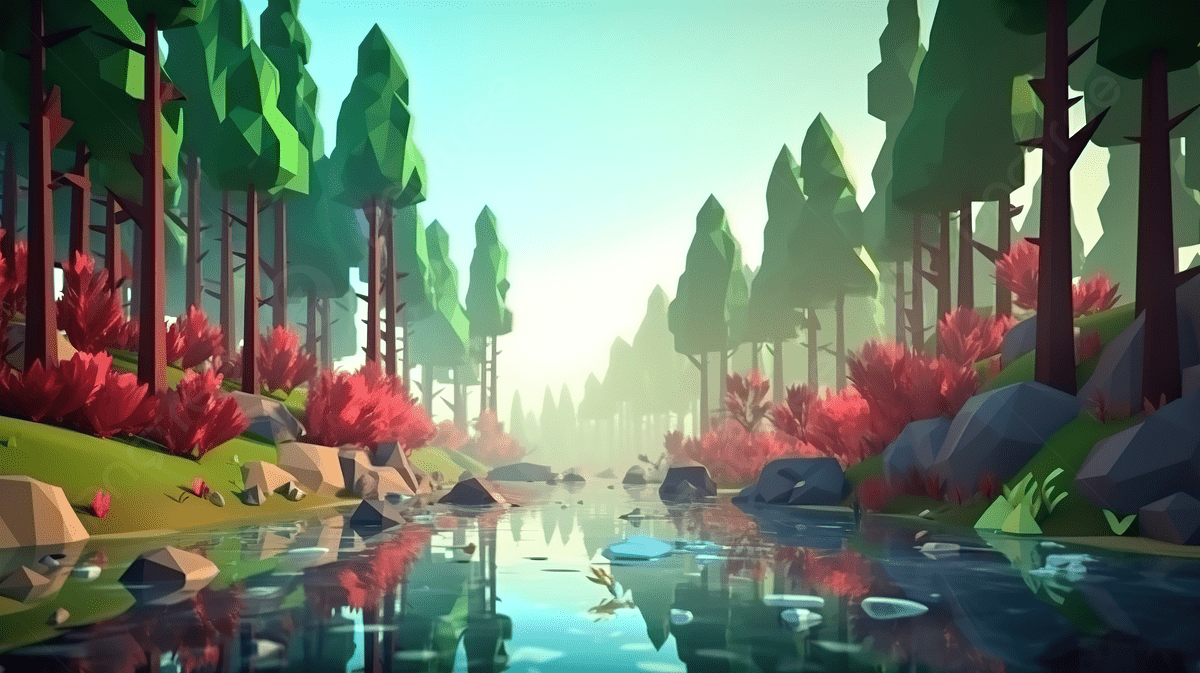
\includegraphics[height = \paperheight]{pics/red_forest.png}
%                 }
%                 ;
%
%                 %% Humidity
%                 \filldraw [white!90!fgcol]
%                 (humidityMarkCenter) circle (\markMainInnerRadius)
%                 ;
%                 \draw [white!90!fgcol, very thick]
%                 (humidityMarkCenter) circle (\markMainOuterRadius)
%                 ;
%                 \draw [use path = markHumeHandle, white!90!fgcol, very thick] ;
%
%                 %% Temperature
%                 \filldraw [white!90!fgcol]
%                 (temperatureMarkCenter) circle (\markMainInnerRadius)
%                 ;
%                 \draw [white!90!fgcol, very thick]
%                 (temperatureMarkCenter) circle (\markMainOuterRadius)
%                 ;
%                 \draw [use path = markTempHandle, white!90!fgcol, very thick] ;
%
%             \end{scope}
%         \end{scope}
%
%         \tikzframetitleleft{Making} {Sense of Data}
%
%         \draw (frametitle.south west) ++(0, -0.5cm) coordinate (content) ;
%         \node [anchor = north west]  (content) at (content) {
%             \begin{minipage} {8.75cm}
%
%                 Every system is in some sense a \alert{Data Processing System}.
%                 They \alert{Convert / Extract / Manipulate} Data in different ways.
%                 There are several kinds of data, such as \alert{Visual}, \alert{Auditory},
%                 \alert{Sensory}, etc. Goal of almost any system is to make the most use of
%                 the data available to it.
%
%             \end{minipage}
%         }
%         ;
%
%         \draw (0, 0)
%         coordinate (origin)
%         (current page.west) coordinate (edge)
%         ;
%         \begin{scope} [transform canvas = {yshift = -2.2cm, xshift = 0.5cm}]
%             \draw []
%             (edge) ++(2cm, -0.5cm) coordinate (pixelMarkCenter)
%             ;
%             \path [name path = markHandle, rounded corners = \markCornerRadius]
%             (pixelMarkCenter) ++(-45:\markMainOuterRadius) coordinate (pixelMarkFirst)
%             (pixelMarkCenter) ++(-45:(1cm + \markMainOuterRadius) coordinate (pixelMarkSecond)
%             (pixelMarkSecond) ++(1, 0) coordinate (pixelMarkThird)
%             (pixelMarkFirst) -- (pixelMarkSecond) -- (pixelMarkThird)
%             ;
%             \draw [use path = markHandle, very thick] ;
%             \filldraw [fgcol]
%             (pixelMarkThird) circle (\markSubRadius)
%             ;
%             \draw [fgcol]
%             (pixelMarkThird) node [right = 6pt] {
%                 Pixel Data
%             }
%             ;
%             \clip [rotate = -45, rounded corners = 0.7cm]
%             (edge) rectangle ++(2.5, 2.5)
%             ;
%             \begin{scope}
%                 \node [anchor = west] (pixel) at (edge) {
%                     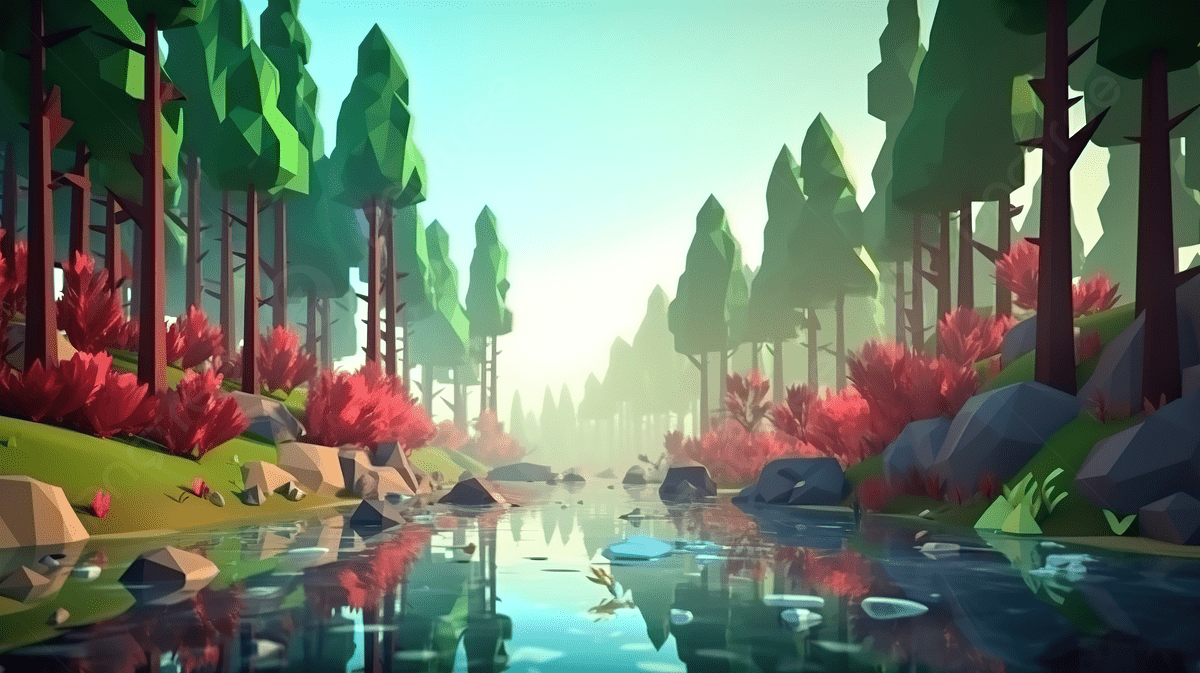
\includegraphics[height = \paperheight]{pics/red_forest.png}
%                 }
%                 ;
%                 \draw [thin, step = 0.1, white, opacity = 0.40]
%                 (edge) ++(-1, -2) grid ++(5, 5)
%                 ;
%                 \filldraw [white!90!fgcol]
%                 (pixelMarkCenter) circle (\markMainInnerRadius)
%                 ;
%
%                 \draw [white!90!fgcol, very thick]
%                 (pixelMarkCenter) circle (\markMainOuterRadius)
%                 ;
%                 \draw [use path = markHandle, white!90!fgcol, very thick] ;
%             \end{scope}
%         \end{scope}
%
%     \end{tikzpicture}
%
% \end{frame}
%
% %% Learning to Ask the Right Questions
% \begin{frame} {}
%
%     \begin{tikzpicture} [
%             remember picture,
%             overlay,
%         ]
%         \tikzframetitleleft{Asking}{The Right Questions}
%
%         \draw (frametitle.south west) ++(0, -0.5cm) coordinate (content) ;
%         \node [anchor = north west]  (content) at (content) {
%             \begin{minipage} {0.45\paperwidth}
%                 In order to make sense of the data, we need to ask the right questions about the data.
%                 The sequence of these questions is known as an \alert{Algorithm}.
%             \end{minipage}
%         }
%         ;
%
%         \filldraw [colorTest]
%         (current page.north east) ++(-7,0) coordinate (workFlowTop)
%         (workFlowTop) rectangle (current page.south east)
%         ;
%
%         \draw (workFlowTop) ++(0, -0.2) coordinate (tmp);
%         \foreach \x in {1, 2, 3, 4} {
%             \draw [very thick, white, rounded corners = 0.2cm, line cap = round]
%             (tmp) ++(0, -1) -- ++(3.5, -0.8) -- ++(3.5, 0.8)
%             (tmp) ++(0, -0.25\paperheight) coordinate (tmp)
%             ;
%         }
%
%         \draw ($(workFlowTop)!0.5!(current page.north east)$) ++(0, -0.8) coordinate (tmp);
%         \foreach \x in {
%             Finding a Problem,
%             Selecting an Algorithm,
%             Implementing the Algorithm,
%             Solving the Problem%
%         } {
%             \draw [ultra thick, white, rounded corners = 0.2cm]
%             (tmp)
%             node [anchor = center] {
%                 \begin{minipage} {7cm}
%                     \centering
%                     \x
%                 \end{minipage}
%             }
%             % (tmp) ++(0, -1) -- ++(3.5, -1.25) -- ++(3.5, 1.25)
%             (tmp) ++(0, -0.25\paperheight) coordinate (tmp)
%             ;
%         }
%
%         %% Methodology
%
%         \begin{scope}
%             \draw
%             (current page.center) ++(1.75cm, 0) coordinate (workFlowMarkCenter)
%             % (current page.center) ++(1.6cm, 0.2cm) coordinate (workFlowMarkCenter)
%             ;
%             \path [name path = markWorkHandle, rounded corners = \markCornerRadius]
%             (workFlowMarkCenter) ++(-180:\markMainOuterRadius) coordinate (workFlowMarkFirst)
%             (workFlowMarkFirst) ++(-1, 0) coordinate (workFlowMarkSecond)
%             (workFlowMarkSecond) ++(-135:0.75cm) coordinate (workFlowMarkThird)
%             (workFlowMarkFirst) -- (workFlowMarkSecond) -- (workFlowMarkThird)
%             ;
%             \draw [use path = markWorkHandle, very thick] ;
%             \filldraw [fgcol]
%             (workFlowMarkThird) circle (\markSubRadius)
%             ;
%             \draw [fgcol]
%             (workFlowMarkThird) node (workFlowMark) [left = 6pt] {
%                 Typical Way of Solving a Problem
%             }
%             ;
%             \clip (workFlowTop) rectangle (current page.south east);
%             \begin{scope}
%                 \filldraw [white!90!fgcol]
%                 (workFlowMarkCenter) circle (\markMainInnerRadius)
%                 ;
%                 \draw [white!90!fgcol, very thick]
%                 (workFlowMarkCenter) circle (\markMainOuterRadius)
%                 ;
%                 \draw [white!90!fgcol, use path = markWorkHandle, very thick] ;
%             \end{scope}
%         \end{scope}
%
%         \draw (content.south west |- workFlowMark.south west) ++(0, -0.5cm) coordinate (content) ;
%         \node [anchor = north west]  (content) at (content) {
%             \begin{minipage} {0.45\paperwidth}
%                 But what if the sheer number of questions one must ask to get to the right answer gets
%                 so overwhelming?
%             \end{minipage}
%         }
%         ;
%
%         \draw (content.south west) ++(0, -0.5cm) coordinate (content) ;
%         \node [anchor = north west]  (content) at (content) {
%             \begin{minipage} {0.45\paperwidth}
%                 But before that...
%             \end{minipage}
%         }
%         ;
%
%     \end{tikzpicture}
%
% \end{frame}
%
% %% Ways of Asking Questions
% \begin{frame}[fragile] {}
%
%     \begin{tikzpicture} [
%             remember picture,
%             overlay
%         ]
%         \tikzframetitleright {Ways of} {Asking Questions}
%
%         \begin{scope} [transform canvas = {xshift = 0.2cm}]
%             \begin{scope}
%                 \draw
%                 (current page.north) ++(-0.75, -0.75) coordinate (ifelseMarkCenter)
%                 ;
%                 \path [name path = ifelseHandle, rounded corners = \markCornerRadius]
%                 (ifelseMarkCenter) ++(-45:\markMainOuterRadius) coordinate (ifelseMarkFirst)
%                 (ifelseMarkCenter) ++(-45:(2.85cm + \markMainOuterRadius) coordinate (ifelseMarkSecond)
%                 (ifelseMarkSecond) ++(1.4, 0) coordinate (ifelseMarkThird)
%                 (ifelseMarkFirst) -- (ifelseMarkSecond) -- (ifelseMarkThird)
%                 ;
%                 \draw [use path = ifelseHandle, very thick] ;
%                 \filldraw [
%                     colorLightGreen,
%                     rounded corners = 0.7cm,
%                 ]
%                 (current page.north west) ++(0, 0.1cm) ++(0,2) coordinate (tmpStart)
%                 (current page.center) ++(0, 0.1cm) coordinate (tmpEnd)
%                 (tmpStart) rectangle (tmpEnd)
%                 ;
%                 \filldraw [fgcol]
%                 (ifelseMarkThird) circle (\markSubRadius)
%                 ;
%                 \draw [fgcol]
%                 (ifelseMarkThird) node (ifelse) [right = 6pt] {
%                     Using If-Else Statements
%                 }
%                 ;
%                 \clip [
%                     rounded corners = 0.7cm,
%                 ]
%                 (current page.north west) ++(0, 0.1cm) ++(0,2) coordinate (tmpStart)
%                 (current page.center) ++(0, 0.1cm) coordinate (tmpEnd)
%                 (tmpStart) rectangle (tmpEnd)
%                 ;
%                 \begin{scope}
%                     \filldraw [white!90!fgcol]
%                     (ifelseMarkCenter) circle (\markMainInnerRadius)
%                     ;
%                     \draw [white!90!fgcol, very thick]
%                     (ifelseMarkCenter) circle (\markMainOuterRadius)
%                     ;
%                     \draw [white!90!fgcol, use path = ifelseHandle, very thick] ;
%                 \end{scope}
%             \end{scope}
%
%             % \draw [thin, step = 0.1, white, opacity = 0.40]
%             % (current page.north west) ++(-2,2) grid (current page.center)
%             % ;
%
%             \begin{scope}
%                 \draw
%                 (current page.south) ++(-0.75, 1.0) coordinate (matrixMarkCenter)
%                 ;
%                 \path [name path = matrixHandle, rounded corners = \markCornerRadius]
%                 (matrixMarkCenter) ++(45:\markMainOuterRadius) coordinate (matrixMarkFirst)
%                 (matrixMarkCenter) ++(45:(2.0cm + \markMainOuterRadius) coordinate (matrixMarkSecond)
%                 (matrixMarkSecond) ++(1.35, 0) coordinate (matrixMarkThird)
%                 (matrixMarkFirst) -- (matrixMarkSecond) -- (matrixMarkThird)
%                 ;
%                 \draw [use path = matrixHandle, very thick] ;
%                 \filldraw [
%                     colorLightSageGreen,
%                     rounded corners = 0.7cm,
%                 ]
%                 (current page.south west) ++(0, -0.1cm) ++(0,-2) coordinate (tmpStart)
%                 (current page.center) ++(0, -0.1cm) coordinate (tmpEnd)
%                 (tmpStart) rectangle (tmpEnd)
%                 ;
%                 \filldraw [fgcol]
%                 (matrixMarkThird) circle (\markSubRadius)
%                 ;
%                 \draw [fgcol]
%                 (matrixMarkThird) node (matrix) [right = 6pt] {
%                     Using Matrix Transformation
%                 }
%                 ;
%                 \clip [
%                     rounded corners = 0.7cm,
%                 ]
%                 (current page.south west) ++(0, -0.1cm) ++(0,-2) coordinate (tmpStart)
%                 (current page.center) ++(0, -0.1cm) coordinate (tmpEnd)
%                 (tmpStart) rectangle (tmpEnd)
%                 ;
%                 \begin{scope}
%                     \filldraw [white!90!fgcol]
%                     (matrixMarkCenter) circle (\markMainInnerRadius)
%                     ;
%                     \draw [white!90!fgcol, very thick]
%                     (matrixMarkCenter) circle (\markMainOuterRadius)
%                     ;
%                     \draw [white!90!fgcol, use path = matrixHandle, very thick] ;
%                 \end{scope}
%             \end{scope}
%
%             % \draw [thin, step = 0.1, white, opacity = 0.40]
%             % (current page.south west) ++(-2,-2) grid (current page.center)
%             % ;
%
%             \draw (current page.north west) ++(0.5cm, -0.5cm) coordinate (content) ;
%             \node [anchor = north west]  (content) at (content) {
%                 \begin{minipage} {0.55\paperwidth}
%                     \begin{minted}[breaklines, autogobble, mathescape] {text}
%                         if this_pixel == this_color:
%                             if this_pixel is at_edge:
%                                 # more and more if statements
%                         elif this_pixel == that_color:
%                             if this_pixel is in_the_middle:
%                                 # many more
%                     \end{minted}
%                 \end{minipage}
%             }
%             ;
%
%             \draw (current page.south west) ++(0.5cm, 0.5cm) coordinate (content) ;
%             \node [anchor = south west]  (content) at (content) {
%                 \begin{minipage} {0.425\paperwidth}
%                     \centering
%                     $\begin{pNiceMatrix}
%                         c_{11} & c_{12} & c_{13} & c_{14} & \cdots & c_{1n} \\
%                         c_{21} & c_{22} & c_{23} & c_{24} & \cdots & c_{2n} \\
%                         c_{31} & c_{32} & c_{33} & c_{34} & \cdots & c_{3n} \\
%                         c_{41} & c_{42} & c_{43} & c_{44} & \cdots & c_{4n} \\
%                         \vdots & \vdots & \vdots & \vdots & \ddots & \vdots\\
%                         c_{m1} & c_{m2} & c_{m3} & c_{m4} & \cdots & c_{mn} \\
%                     \end{pNiceMatrix}$
%                 \end{minipage}
%             }
%             ;
%
%         \end{scope}
%
%         \draw (ifelse.south east) ++(0.2cm, -0.5cm) coordinate (content) ;
%         \node [anchor = north east]  (content) at (content) {
%             \begin{minipage} {6.5cm}
%                 There are several ways to ask the same question. One might be able to
%                 to write an Algorithm for parsing the pixel data just by using \alert{If-Else}
%                 statements.
%             \end{minipage}
%         }
%         ;
%
%         \draw (matrix.south east) ++(0.2cm, -0.5cm) coordinate (content) ;
%         \node [anchor = north east]  (content) at (content) {
%             \begin{minipage} {6.5cm}
%                 Or one can directly transform input into output using a \alert{Matrix Tranformation}.
%             \end{minipage}
%         }
%         ;
%
%     \end{tikzpicture}
%
% \end{frame}
%
% %% Guess Who's Good at Crunching Matrices?
% \begin{frame} {}
%
%     \begin{tikzpicture} [
%             remember picture,
%             overlay
%         ]
%
%         \tikzframetitleright{Guess Who's} {Good at Crunching Matrices?}
%
%         \draw (0, 0)
%         coordinate (origin)
%         (current page.south west) coordinate (edge)
%         ;
%
%         \begin{scope} [
%                 transform canvas = {
%                     yshift = -13,
%                     xshift = -13,
%                 }
%             ]
%             \begin{scope} [
%                     transform canvas = {
%                         yshift = 0.1cm,
%                         xshift = 0.1cm,
%                     }
%                 ]
%                 \draw
%                 (current page.north) ++(-2.0, -1.6) coordinate (cpuMarkCenter)
%                 ;
%                 \path [name path = cpuHandle, rounded corners = \markCornerRadius]
%                 (cpuMarkCenter) ++(0:\markMainOuterRadius) coordinate (cpuMarkFirst)
%                 (cpuMarkCenter) ++(0:(1.5cm + \markMainOuterRadius) coordinate (cpuMarkSecond)
%                 (cpuMarkSecond) ++(-45:2.1cm) coordinate (cpuMarkThird)
%                 (cpuMarkThird) ++(5, 0) coordinate (cpuMarkFourth)
%                 (cpuMarkFirst) -- (cpuMarkSecond) -- (cpuMarkThird) -- (cpuMarkFourth)
%                 ;
%                 \draw [use path = cpuHandle, very thick] ;
%                 \filldraw [fgcol]
%                 (cpuMarkFourth) circle (\markSubRadius)
%                 ;
%                 \draw [fgcol]
%                 (cpuMarkFourth) node (cpu) [right = 6pt] {
%                     CPUs
%                 }
%                 ;
%                 \begin{scope}
%                     \clip [rotate = 45, rounded corners = 0.7cm]
%                     (edge) ++(0.25, 0.25) rectangle ++(10, 10)
%                     ;
%                     \draw
%                     (edge) ++(3.00, 0.35) coordinate (tmp)
%                     ;
%                     \node [anchor = south] (img) at (tmp) {
%                         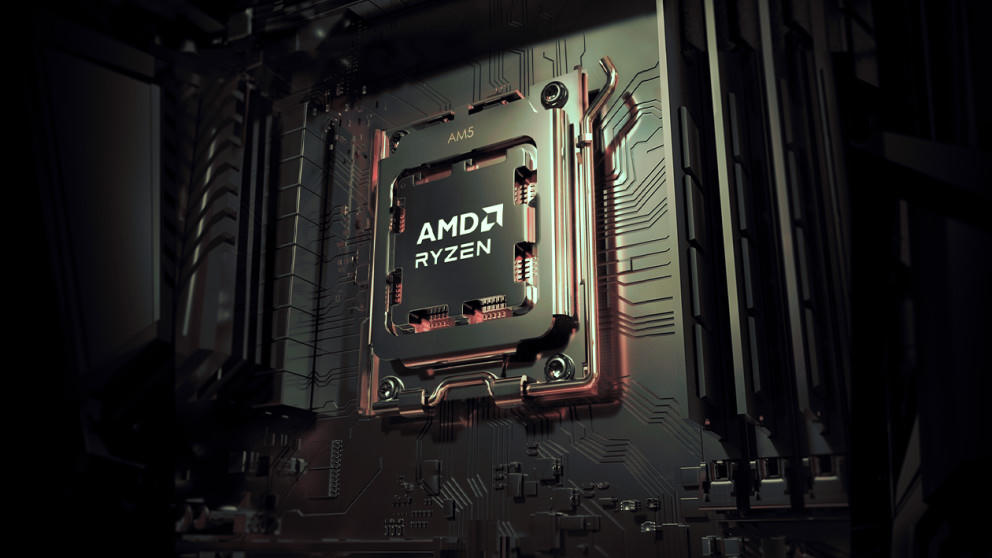
\includegraphics[height = \paperheight]{pics/cpu.png}
%                     }
%                     ;
%                     \filldraw [white!90!fgcol]
%                     (cpuMarkCenter) circle (\markMainInnerRadius)
%                     ;
%                     \draw [white!90!fgcol, very thick]
%                     (cpuMarkCenter) circle (\markMainOuterRadius)
%                     ;
%                     \draw [white!90!fgcol, use path = cpuHandle, very thick] ;
%                 \end{scope}
%
%                 \draw (cpu.south east) ++(0, -0.3cm) coordinate (content) ;
%                 \node [anchor = north east]  (content) at (content) {
%                     \begin{minipage} {6.0cm}
%                         \raggedleft
%                         \alert{CPUs} are much more capable at processing matrices that anyone of us, humans.
%                         % \alert{Computers}, especially \alert{GPUs} can crunch through matrices.
%                     \end{minipage}
%                 }
%                 ;
%             \end{scope}
%
%             \begin{scope} [
%                     transform canvas = {
%                         yshift = -0.5cm,
%                         xshift = -0.5cm,
%                     }
%                 ]
%                 \draw
%                 (current page.south) ++(1.75, 3.25) coordinate (gpuMarkCenter)
%                 ;
%                 \path [name path = gpuHandle, rounded corners = \markCornerRadius]
%                 (gpuMarkCenter) ++(45:\markMainOuterRadius) coordinate (gpuMarkFirst)
%                 (gpuMarkCenter) ++(45:(1.0cm + \markMainOuterRadius) coordinate (gpuMarkSecond)
%                 (gpuMarkSecond) ++(4.25, 0) coordinate (gpuMarkThird)
%                 (gpuMarkFirst) -- (gpuMarkSecond) -- (gpuMarkThird)
%                 ;
%                 \draw [use path = gpuHandle, very thick] ;
%                 \filldraw [fgcol]
%                 (gpuMarkThird) circle (\markSubRadius)
%                 ;
%                 \draw [fgcol]
%                 (gpuMarkThird) node (gpu) [right = 6pt] {
%                     GPUs
%                 }
%                 ;
%                 \begin{scope}
%                     \clip [rotate = 45, rounded corners = 0.7cm]
%                     (edge) ++(0.25, -0.25) rectangle ++(10, -10)
%                     ;
%                     \draw
%                     (edge) ++(0, -0.5) coordinate (tmp)
%                     ;
%                     \node [anchor = south west] (img) at (tmp) {
%                         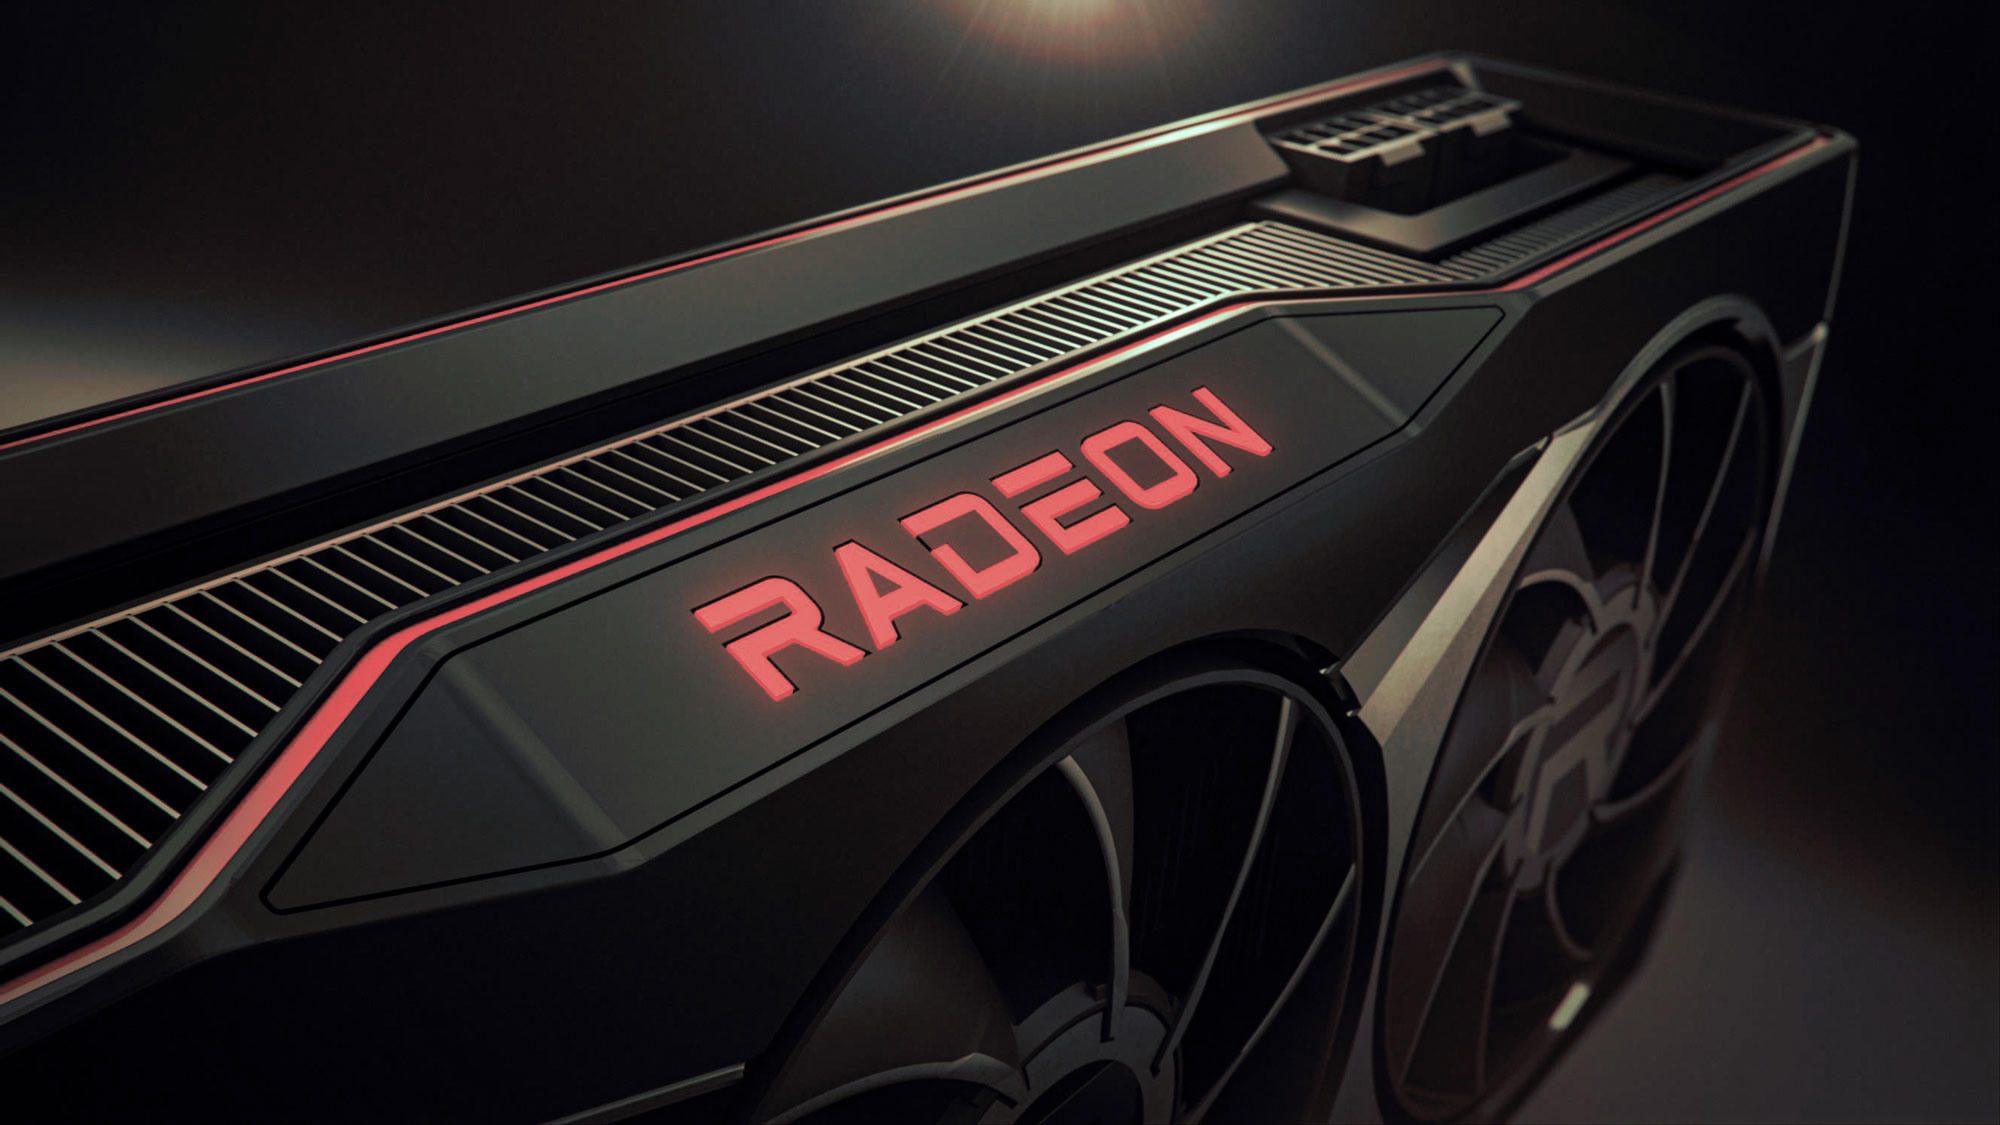
\includegraphics[height = 0.9\paperheight]{pics/gpu.png}
%                     }
%                     ;
%                     \filldraw [white!90!fgcol]
%                     (gpuMarkCenter) circle (\markMainInnerRadius)
%                     ;
%                     \draw [white!90!fgcol, very thick]
%                     (gpuMarkCenter) circle (\markMainOuterRadius)
%                     ;
%                     \draw [white!90!fgcol, use path = gpuHandle, very thick] ;
%                 \end{scope}
%                 \draw (gpu.south east) ++(0, -0.3cm) coordinate (content) ;
%                 \node [anchor = north east]  (content) at (content) {
%                     \begin{minipage} {4.0cm}
%                         \raggedleft \alert{GPUs} can exploit parallelizable nature of matrix operations.
%                         % \alert{Computers}, especially \alert{GPUs} can crunch through matrices.
%                     \end{minipage}
%                 }
%                 ;
%             \end{scope}
%         \end{scope}
%
%     \end{tikzpicture}
%
%
% \end{frame}
%
% %% Learning to Ask Questions
% \begin{frame} {}
%
%     \begin{tikzpicture} [
%             remember picture,
%             overlay
%         ]
%
%         \tikzframetitleleft{Learning to} {Ask Questions}
%
%         \draw (0, 0)
%         coordinate (origin)
%         (current page.north east) coordinate (edge)
%         ;
%
%         \begin{scope} [
%                 transform canvas = {
%                     yshift = -0.5cm,
%                     xshift = -1.25cm,
%                 }
%             ]
%             \begin{scope}
%                 \clip [rotate = -45, rounded corners = 0.7cm]
%                 (edge) ++(7, 6) rectangle ++(-12, -12)
%                 ;
%                 \draw
%                 (edge) ++(-2, 0.625) coordinate (tmp)
%                 ;
%                 \node [anchor = north] (img) at (tmp) {
%                     
\includegraphics[height = \paperheight]{pics/snetwork.png}
%                 }
%                 ;
%             \end{scope}
%
%         \end{scope}
%
%         \draw (frametitle.south west) ++(0, -0.3cm) coordinate (content) ;
%         \node [anchor = north west]  (content) at (content) {
%             \begin{minipage} {6.8cm}
%                 We haven't addressed how we are going to know the right questions to ask about
%                 a data yet.
%             \end{minipage}
%         }
%         ;
%
%         \draw (content.south west) ++(0, -0.3cm) coordinate (content) ;
%         \node [anchor = north west]  (content) at (content) {
%             \begin{minipage} {8.1cm}
%                 The \alert{coefficients / weights} in our question matrix decides the output
%                 we get.
%             \end{minipage}
%         }
%         ;
%
%         \draw (content.south west) ++(0, -0.3cm) coordinate (content) ;
%         \node [anchor = north west]  (content) at (content) {
%             \begin{minipage} {9.3cm}
%                 And the game of finding these coefficients / weights is famously known under
%                 the umbrella term \alert{Machine Learning}.
%             \end{minipage}
%         }
%         ;
%
%     \end{tikzpicture}
%
% \end{frame}
%
% %% Weight of the Ever Growing Data
% \begin{frame} {}
%
%     \begin{tikzpicture} [
%             remember picture,
%             overlay
%         ]
%         \tikzframetitleleft{Weight of} {The Ever Growing Data}
%
%         \begin{scope} [
%                 rotate = 45,
%                 transform canvas = {
%                     yshift = -1.1cm,
%                 },
%             ]
%             \draw ($(current page.center)!0.3!(current page.east)$) coordinate (power);
%
%             \begin{scope}
%                 \path [name path = mountainHandle, rounded corners = 0.7cm]
%                 (power) ++(-2.5, -2.5) rectangle ++(5, 5)
%                 ;
%                 \clip[use path = mountainHandle] ;
%                 \begin{scope}
%                     \node [anchor = center] (pixel) at (power) {
%                         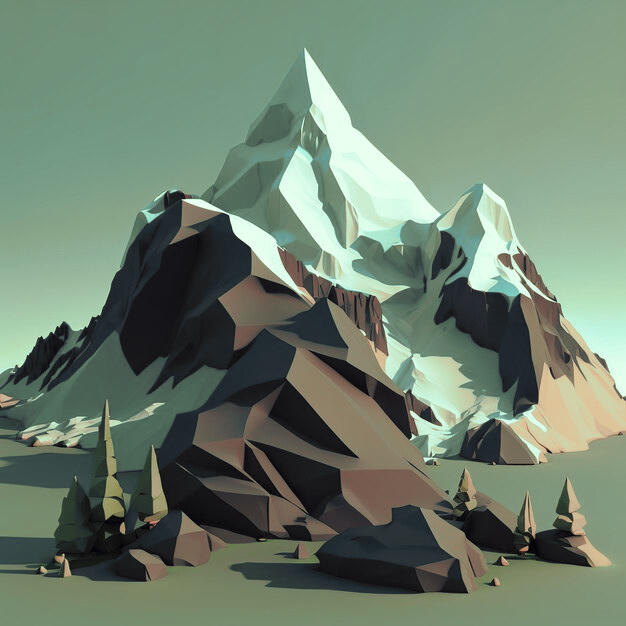
\includegraphics[height = 0.75\paperheight]{pics/mountain.png}
%                     }
%                     ;
%                 \end{scope}
%             \end{scope}
%
%             \draw (power) ++(5.5, 0) coordinate (power);
%
%             \begin{scope}
%                 \path [name path = powerHandle, rounded corners = 0.7cm]
%                 (power) ++(-2.5, -2.5) rectangle ++(5, 5)
%                 ;
%                 \clip[use path = powerHandle] ;
%                 \begin{scope}
%                     \node [anchor = center] (pixel) at (power) {
%                         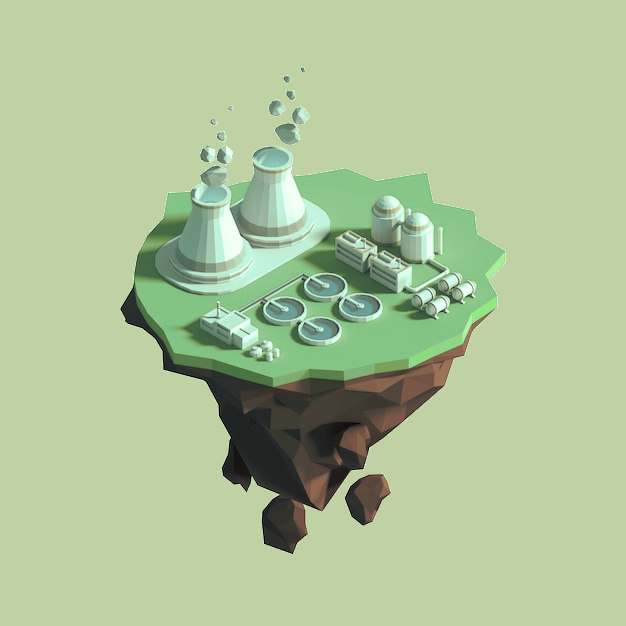
\includegraphics[height = 0.75\paperheight]{pics/power.png}
%                     }
%                     ;
%                 \end{scope}
%             \end{scope}
%
%             \draw (power) ++(-5.5, -5.5) coordinate (power);
%
%             \begin{scope}
%                 \path [name path = cloudHandle, rounded corners = 0.7cm]
%                 (power) ++(-2.5, -2.5) rectangle ++(5, 5)
%                 ;
%                 \clip[use path = cloudHandle] ;
%                 \begin{scope}
%                     \node [anchor = center] (pixel) at (power) {
%                         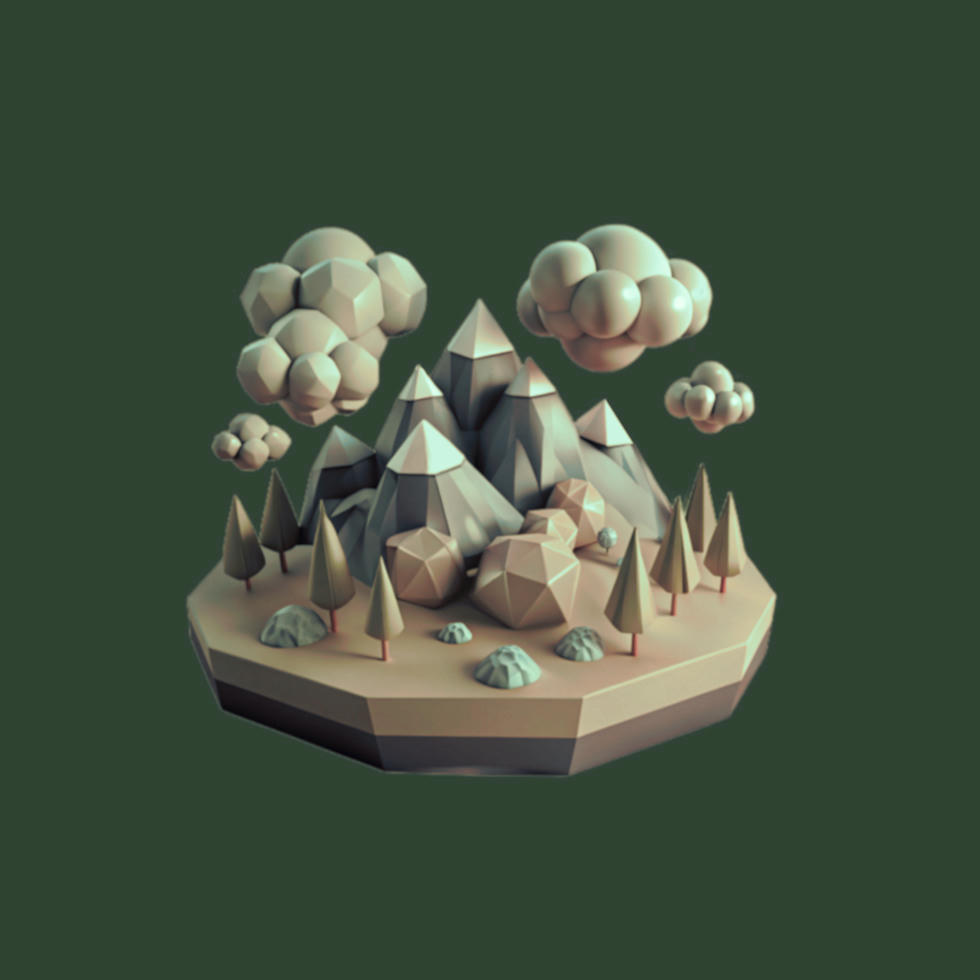
\includegraphics[height = 0.75\paperheight]{pics/cloud.png}
%                     }
%                     ;
%                 \end{scope}
%             \end{scope}
%
%             % \draw (power) ++(5.5, 0) coordinate (power);
%             %
%             % \filldraw [rounded corners = 0.7cm]
%             % (power) ++(-2.5, -2.5) rectangle ++(5, 5)
%             % ;
%
%         \end{scope}
%
%         \draw (frametitle.south west) ++(0, -0.3cm) coordinate (content) ;
%         \node [anchor = north west]  (content) at (content) {
%             \begin{minipage} {6.5cm}
%                 Day by day ML Models are getting more and more capabilities.
%                 So as the need for more and more powerful hardware to run these models.
%
%                 This can lead to several concerns:
%
%                 \begin{itemize}
%                     \item Increased Carbon Footprint.
%                     \item Reliance of Cloud Computing.
%                     \item Latency related with Cloud Computing.
%                     \item Need for powerful Hardware.
%                 \end{itemize}
%
%                 \alert{TinyML} is a subset of ML that is trying to address these issues.
%
%             \end{minipage}
%         }
%         ;
%
%     \end{tikzpicture}
%
% \end{frame}
%
% %% An Introduction to Tiny Machine Learning
% \begin{frame} {}
%
%     \begin{tikzpicture} [
%             remember picture,
%             overlay
%         ]
%
%         \tikzframetitleright{An Introduction to} {Tiny Machine Learning}
%
%         \draw (frametitle.south east) ++(0, -0.3cm) coordinate (content) ;
%         \node [anchor = north east]  (content) at (content) {
%             \begin{minipage} {0.5\textwidth}
%
%                 TinyML is a subset of machine learning (ML) that focuses on developing and deploying
%                 ML models on resource-constrained devices such as:
%
%                 \begin{itemize}
%                     \item Microcontrollers (MCUs)
%                     \item System-on-Chip (SoCs)
%                     \item FPGAs
%                 \end{itemize}
%
%             \end{minipage}
%         }
%         ;
%
%         \def\picWidth{7}
%         \def\picGap{0.6cm}
%
%         \draw [
%             rounded corners = 0.7cm,
%         ]
%
%         ($(current page.center)!0.5!(current page.west)$) coordinate (picCenter)
%
%         % (picCenter) ++(-\picWidth / 2, -\picWidth / 2) rectangle ++(\picWidth, \picWidth)
%
%         (picCenter) ++(-\picWidth / 2, -\picWidth / 2)
%         coordinate (picCenterLeft)
%
%         (picCenter) ++(\picWidth / 2, \picWidth / 2)
%         coordinate (picCenterRight)
%
%         (current page.north -| picCenterLeft) ++(0, 1) coordinate (picTopLeft)
%         (current page.north -| picCenterRight) ++(0, 1) coordinate (picTopRight)
%
%         (current page.south -| picCenterLeft) ++(0, -1) coordinate (picBotLeft)
%         (current page.south -| picCenterRight) ++(0, -1) coordinate (picBotRight)
%
%         ;
%
%         \path [
%             name path = topPic,
%             rounded corners = 0.7cm,
%         ]
%         (picCenterLeft) -- (picTopLeft) -- (picTopRight) -- (picCenterRight) -- cycle
%         ;
%
%         \path [
%             name path = botPic,
%             rounded corners = 0.7cm,
%         ]
%         (picCenterLeft) -- (picBotLeft) -- (picBotRight) -- (picCenterRight) -- cycle
%         ;
%
%         \begin{scope} [
%                 transform canvas = {
%                     xshift = -0.2cm,
%                     yshift = -0.2cm,
%                 },
%             ]
%             \begin{scope} [
%                     transform canvas = {
%                         yshift = \picGap/2,
%                     },
%                 ]
%
%                 \clip [use path = topPic] ;
%
%                 \draw
%                 (current page.north west)
%                 ++(-0.25, 0)
%                 node [anchor = north west] (img) {
%                     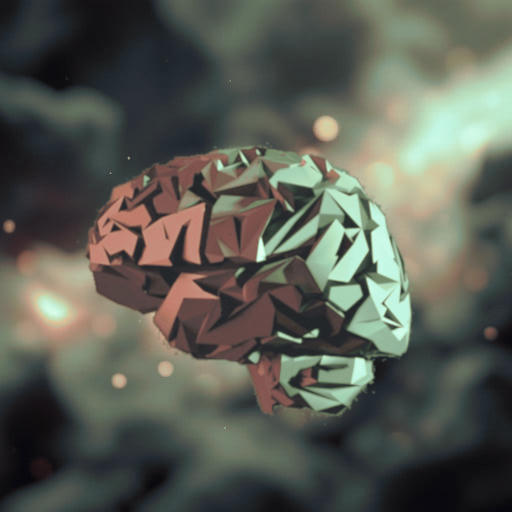
\includegraphics[height = 0.85\paperheight]{pics/brain.png}
%                 }
%                 ;
%
%             \end{scope}
%
%
%             \begin{scope} [
%                     transform canvas = {
%                         yshift = -\picGap/2,
%                     },
%                 ]
%
%                 \clip [use path = botPic] ;
%
%                 \draw
%                 (current page.south west)
%                 node [anchor = south west] (img) {
%                     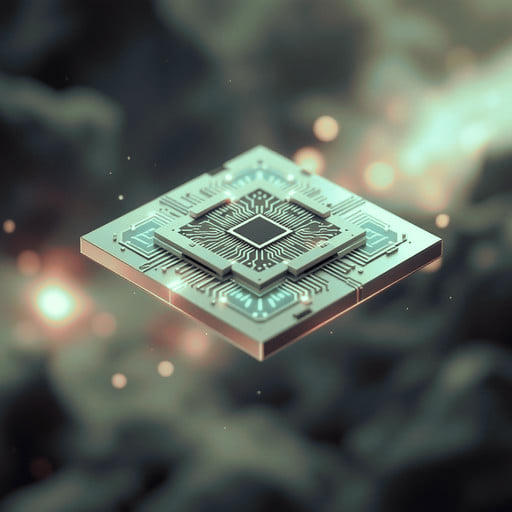
\includegraphics[height = 0.85\paperheight]{pics/chip.png}
%                 }
%                 ;
%
%             \end{scope}
%
%         \end{scope}
%
%
%     \end{tikzpicture}
% \end{frame}
%
% %% Why Even Run Machine Learning Models on Microcontrollers?
% \begin{frame}
%
%     \begin{tikzpicture} [
%             remember picture,
%             overlay,
%         ]
%
%         \tikzframetitleright{Why Even Run} {Machine Learning Models on Microcontrollers?}
%
%         \filldraw
%         ($(current page.center)!0.5!(current page.west)$) ++(3.25cm, -3.5cm) coordinate (center)
%         ;
%
%         \subSquare{s1}{center}{padBotCorner} % second
%         \subSquare{s2}{center}{padLeftCorner} % third
%         \subSquare{s3}{center}{padRightCorner} % first
%         \subSquare{s4}{s2-padRightCorner}{padBotCorner} % fourth
%
%         \drawSubSquare{colorLightGreen,}{s1}
%         \drawSubSquare{colorLightSageGreen,}{s2}
%         \drawSubSquare{colorLightSageGreen,}{s3}
%         \drawSubSquare{colorLightGreen,}{s4}
%
%         \node [anchor = center] at (s1-center) {
%             \begin{minipage} {\squareSide}
%                 \centering
%                 \large Privacy and Security
%             \end{minipage}
%         }
%         ;
%         \node [anchor = center] at (s3-center) {
%             \begin{minipage} {\squareSide}
%                 \centering
%                 \large Low Power \\ Consumption
%             \end{minipage}
%         }
%         ;
%         \node [anchor = center] at (s2-center) {
%             \begin{minipage} {\squareSide}
%                 \centering
%                 \large Improved \\ Latency
%             \end{minipage}
%         }
%         ;
%         \node [anchor = center] at (s4-center) {
%             \begin{minipage} {\squareSide}
%                 \centering
%                 \large Economically \\ Viable
%             \end{minipage}
%         }
%         ;
%
%         \def\picSide{8}
%
%         \begin{scope} [
%                 transform canvas = {
%                     yshift = -0.25cm,
%                     xshift = -2.75cm,
%                 },
%                 rotate = -45,
%             ]
%             \clip [
%                 rounded corners = 0.7cm,
%             ]
%             (current page.north west)
%             ++(0, \picSide/2)
%             rectangle ++(\picSide, -\picSide)
%             ;
%
%             \draw
%             (current page.north west) ++(-5cm, 0)
%             node (img) [anchor = north west, inner sep = 0pt] {
%                 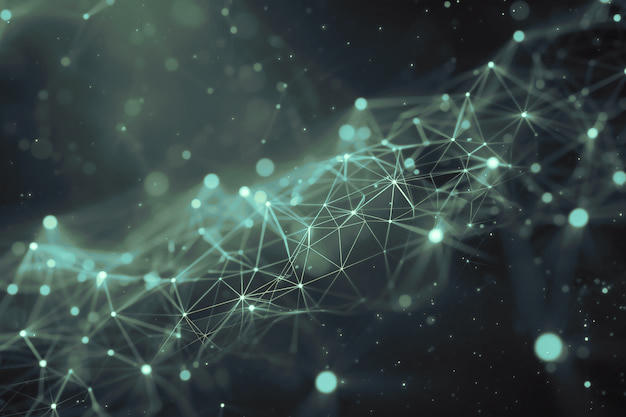
\includegraphics[height = \paperwidth] {pics/bnet.png}
%             }
%             ;
%
%         \end{scope}
%
%     \end{tikzpicture}
%
% \end{frame}
%
% %% Privacy and Security
% \begin{frame} {}
%
%
%     \begin{tikzpicture} [
%             remember picture,
%             overlay,
%         ]
%
%         \tikzframetitleleft{Privacy} {And Security}
%
%         \def\picSide{7cm}
%
%         \begin{scope}
%             \clip[
%                 rounded corners = 0.7cm,
%             ]
%             ($(current page.center)!0.5!(current page.east)$)
%             ++(-0.75, 0)
%             coordinate (center)
%
%             (center) ++(-\picSide/2, -\picSide/2) rectangle ++(\picSide, \picSide)
%
%             ;
%
%             \draw
%             (center) ++(-0.75, 0)
%             node [anchor = center, inner sep = 0pt] {
%                 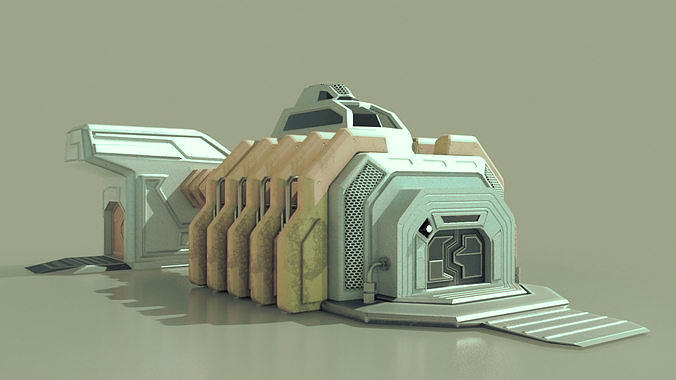
\includegraphics[height = 0.8\paperheight]{pics/military_base.png}
%             }
%             ;
%         \end{scope}
%
%
%         \draw
%         ($(current page.south)!0.5!(current page.south |- frametitle.south)$)
%         coordinate (contentCenter)
%         (frametitle.west |- contentCenter)
%         node [anchor = west] {
%             \begin{minipage} {0.425\textwidth}
%
%                 \begin{center}
%                     ``The most secure connection is no connection at all."
%                 \end{center}
%
%                 \begin{itemize}
%                     \item That is the beauty of \alert{Edge Computing}, everything stays
%                         locally on the device itself.
%
%                     \item Since the ML Model is running on
%                         the device itself, there is no need sent anything over the wire
%                         or air.
%
%                     \item This provides the most security and privacy.
%                 \end{itemize}
%
%             \end{minipage}
%         }
%         ;
%
%     \end{tikzpicture}
%
% \end{frame}
%
% %% Economically Viable
% \begin{frame} {}
%
%     \begin{tikzpicture} [
%             remember picture,
%             overlay,
%         ]
%
%         \tikzframetitleleft{Economically} {Viable}
%
%         \def\picSide{7cm}
%
%         \begin{scope}
%             \clip[
%                 rounded corners = 0.7cm,
%             ]
%             ($(current page.center)!0.5!(current page.east)$)
%             ++(-0.75, 0)
%             coordinate (center)
%
%             (center) ++(-\picSide/2, -\picSide/2) rectangle ++(\picSide, \picSide)
%
%             ;
%             \draw
%             (center)
%             node [anchor = center, inner sep = 0pt] {
%                 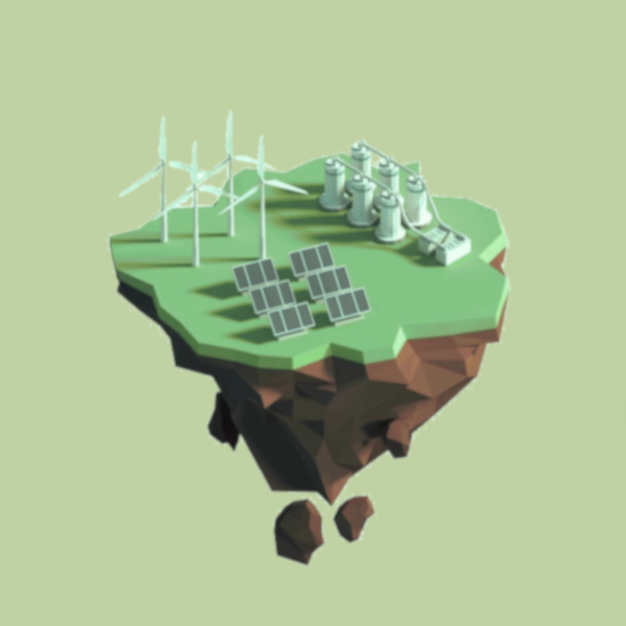
\includegraphics[height = 0.8\paperheight]{pics/renew.png}
%             }
%             ;
%         \end{scope}
%
%         \draw
%         ($(current page.south)!0.5!(current page.south |- frametitle.south)$)
%         coordinate (contentCenter)
%         (frametitle.west |- contentCenter)
%         ++(0, 0.5)
%         node [anchor = west] {
%             \begin{minipage} {0.425\textwidth}
%
%                 \begin{itemize}
%                     \item Modern day Microcontrollers are \alert{extremely cheap}.
%                     \item And they are literally used everywhere.
%                     % \item So it is highly economical to use these tiny devices than
%                     %     to use other \alert{expensive devices}.
%                 \end{itemize}
%
%                 \begin{center}
%                     \begin{tabularx} {\textwidth} {
%                             >{\centering \arraybackslash}m{0.6\textwidth}
%                             >{\centering \arraybackslash}X
%                         }
%                         \toprule
%
%                         Microcontroller & Price \\ \midrule
%
%                         ESP32 & 550 \\
%
%                         Arduino UNO &  570 \\
%
%                         Raspberry Pi Pico & 450 \\
%
%                         \bottomrule
%
%                     \end{tabularx}
%                 \end{center}
%
%             \end{minipage}
%         }
%         ;
%
%     \end{tikzpicture}
%
% \end{frame}
%
% %% Low Power Consumption
% \begin{frame} {}
%
%     \begin{tikzpicture} [
%             remember picture,
%             overlay,
%         ]
%
%         \tikzframetitleright{Low Power} {Consumption}
%
%         \def\picSide{7cm}
%
%         \begin{scope}
%             \clip[
%                 rounded corners = 0.7cm,
%             ]
%             ($(current page.center)!0.5!(current page.west)$)
%             ++(0.75, 0)
%             coordinate (center)
%
%             (center) ++(-\picSide/2, -\picSide/2) rectangle ++(\picSide, \picSide)
%
%             ;
%             \draw
%             (center)
%             ++(1.25, 0)
%             node [anchor = center, inner sep = 0pt] {
%                 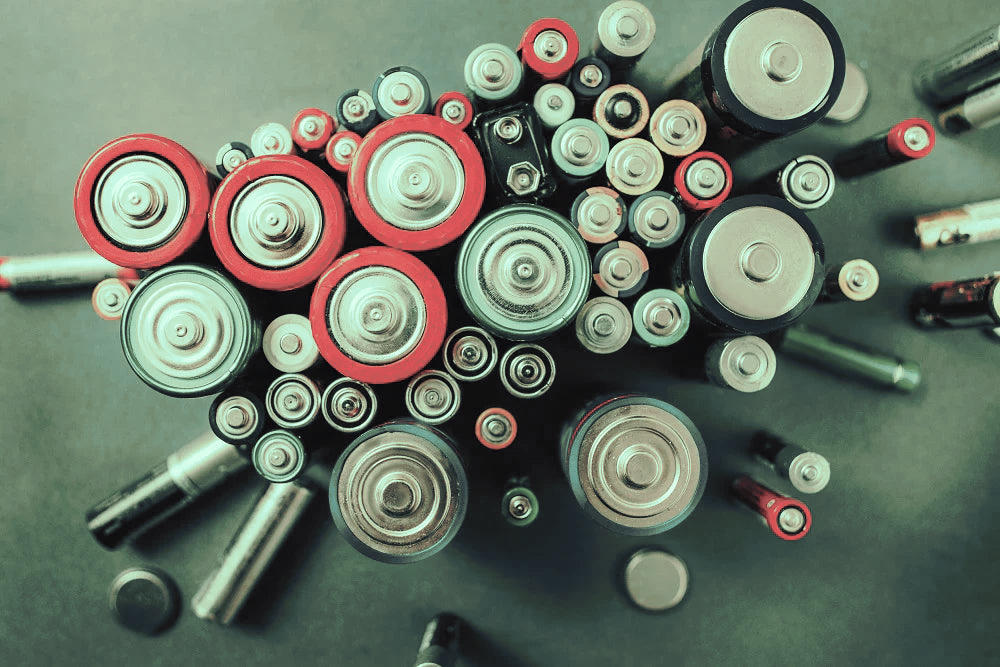
\includegraphics[height = 0.8\paperheight]{pics/battery.png}
%             }
%             ;
%         \end{scope}
%
%         \draw
%         ($(current page.south)!0.5!(current page.south |- frametitle.south)$)
%         coordinate (contentCenter)
%         (frametitle.east |- contentCenter)
%         ++(0, 0.5)
%         node [anchor = east] {
%             \begin{minipage} {0.425\textwidth}
%
%                 \begin{itemize}
%                     \item Modern day Microcontrollers are \alert{extremely power efficient}.
%                     \item While a Raspberry Pi 4 can draw around 1.5A.
%                     % \item So it is highly economical to use these tiny devices than
%                     %     to use other \alert{expensive devices}.
%                 \end{itemize}
%
%                 \begin{center}
%                     \begin{tabularx} {\textwidth} {
%                             >{\centering \arraybackslash}X
%                             >{\centering \arraybackslash}m{0.4\textwidth}
%                         }
%                         \toprule
%
%                         Microcontroller & Current Consumption \\ \midrule
%
%                         ESP32 & 20-60 mA \\
%
%                         Arduino UNO & 45-80 mA \\
%
%                         Raspberry Pi Pico & 18-50 mA \\
%
%                         \bottomrule
%
%                     \end{tabularx}
%                 \end{center}
%
%             \end{minipage}
%         }
%         ;
%     \end{tikzpicture}
%
% \end{frame}
%
% %% Improved Latency
% \begin{frame} {}
%
%     \begin{tikzpicture} [
%             remember picture,
%             overlay,
%         ]
%
%         \tikzframetitleright{Improved} {Latency}
%
%         \def\picSide{7cm}
%
%         \begin{scope}
%             \clip[
%                 rounded corners = 0.7cm,
%             ]
%             ($(current page.center)!0.5!(current page.west)$)
%             ++(0.75, 0)
%             coordinate (center)
%
%             (center) ++(-\picSide/2, -\picSide/2) rectangle ++(\picSide, \picSide)
%
%             ;
%             \draw
%             (center)
%             ++(-1.5, 0)
%             node [anchor = center, inner sep = 0pt] {
%                 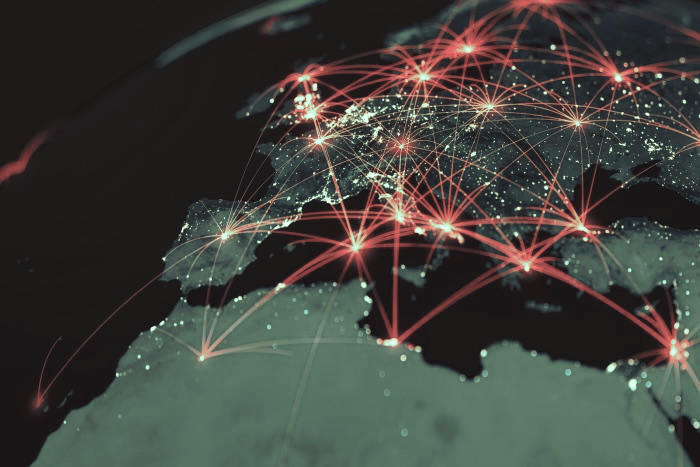
\includegraphics[height = 0.8\paperheight]{pics/latency.png}
%             }
%             ;
%         \end{scope}
%
%         \draw
%         ($(current page.south)!0.5!(current page.south |- frametitle.south)$)
%         coordinate (contentCenter)
%         (frametitle.east |- contentCenter)
%         ++(0, 0.5)
%         node [anchor = east] {
%             \begin{minipage} {0.425\textwidth}
%
%                 \begin{itemize}
%                     \item No need for cloud processing.
%
%                     \item Everything is \alert{processed locally}.
%
%                     \item So zero network latency.
%
%                     \item Can be deployed to \alert{remote location}.
%                 \end{itemize}
%
%             \end{minipage}
%         }
%         ;
%
%     \end{tikzpicture}
%
% \end{frame}
%
% %% The 14 Kilo-Byte "Ok Google" ML Model
% \begin{frame} {}
%
%     \begin{tikzpicture} [
%             remember picture,
%             overlay,
%         ]
%
%         \tikzframetitleleft{The 14 Kilo-Byte} {``Ok Google" ML Model}
%
%         \draw (frametitle.south west) ++(0, -0.3cm) coordinate (content) ;
%         \node [anchor = north west]  (content) at (content) {
%             \begin{minipage} {8.0cm}
%
%                 In 2014, Engineers at Google had to implement the ``Ok Google"
%                 waking feature. But they couldn't use the main CPU for this, as
%                 it was powered off to conserve battery. So they developed a
%                 \alert{14 kilo-byte (KB)} neural network that ran on an embedded
%                 DSPs that had only \alert{tens of kilo-bytes of memory}!
%
%                 \vspace{0.5cm}
%
%                 \begin{minipage} {6.5cm}
%
%                     These specialised DSPs
%                     only used \alert{few milliwatts (mW) of power}.
%
%                 \end{minipage}
%             \end{minipage}
%
%         }
%         ;
%
%         \draw (0, 0)
%         coordinate (origin)
%         (current page.east) ++(1, 0) coordinate (edge)
%         ;
%
%         \begin{scope}
%
%             \draw [
%                 name path = contentHandle,
%             ]
%             (content.south) ++(-2.75, -0.3) coordinate (contentMarkEnd)
%             (contentMarkEnd) ++(-45:1) coordinate (contentMarkThird)
%             (contentMarkThird) ++(7.5, 0) coordinate (contentMarkSecond)
%             (contentMarkSecond) ++(45:1) coordinate (contentMarkFirst)
%             (contentMarkFirst) ++(45:\markMainOuterRadius) coordinate (contentMarkCenter)
%             (contentMarkFirst) -- (contentMarkSecond) -- (contentMarkThird) -- (contentMarkEnd)
%             ;
%
%             \draw [use path = contentHandle, very thick] ;
%             ;
%             \filldraw [fgcol]
%             (contentMarkEnd) circle (\markSubRadius)
%             ;
%
%             \clip [rotate = 45, rounded corners = 0.7cm]
%             (edge) ++(-10, -15) rectangle ++(20, 20)
%             ;
%
%             \begin{scope}
%                 \draw
%                 (edge) ++(5, 0)
%                 node [anchor = east] (img) {
%                     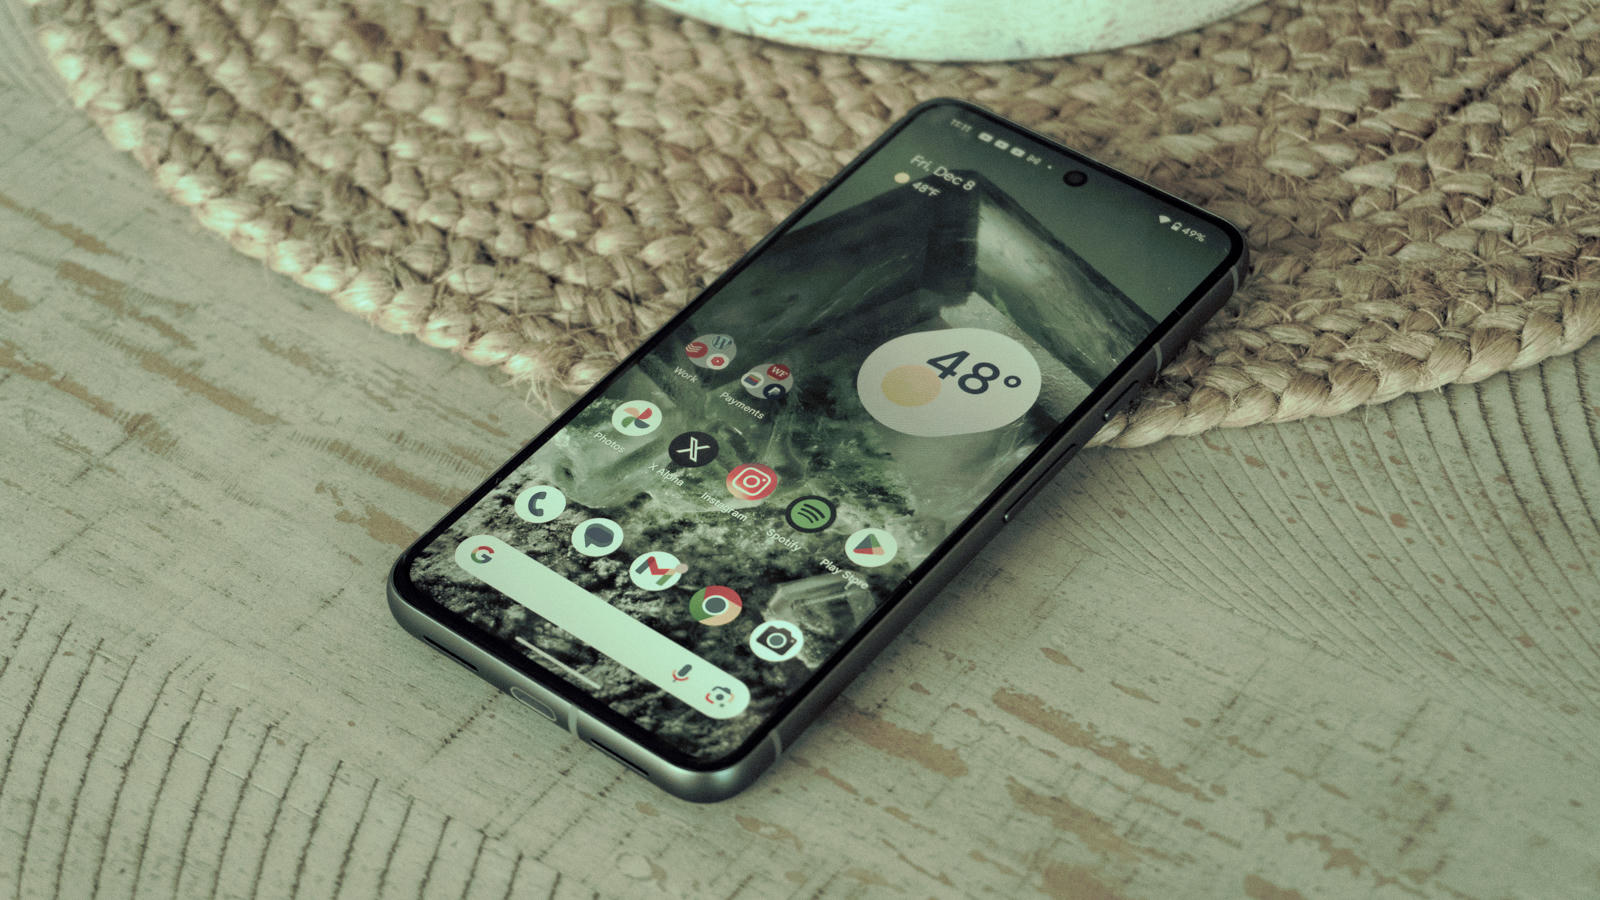
\includegraphics[height = \paperheight]{pics/phone.png}
%                 }
%                 ;
%
%                 \filldraw [white!90!fgcol]
%                 (contentMarkCenter) circle (\markMainInnerRadius)
%                 ;
%                 \draw [white!90!fgcol, very thick]
%                 (contentMarkCenter) circle (\markMainOuterRadius)
%                 ;
%                 \draw [use path = contentHandle, white!90!fgcol, very thick] ;
%             \end{scope}
%         \end{scope}
%
%     \end{tikzpicture}
%
% \end{frame}
%
% % Comparing Modern Day Microcontrollers
% \begin{frame} {}
%
%     \begin{tikzpicture} [
%             remember picture,
%             overlay,
%         ]
%
%         \tikzframetitlelongleft{Comparing}{Modern Day Microcontrollers}
%
%         \draw (frametitle.south west) ++(0, -0.1cm) coordinate (content) ;
%         \node [anchor = north west]  (content) at (content) {
%             \begin{minipage} {\textwidth}
%
%                 \centering
%
%                 \begin{tabularx} {\textwidth} {
%                         >{\centering \arraybackslash}X
%                         >{\centering \arraybackslash}X
%                         >{\centering \arraybackslash}X
%                         >{\centering \arraybackslash}X
%                         >{\centering \arraybackslash}X
%                     }
%
%                     \toprule
%
%                     \multicolumn{2}{c}{Microcontroller} & Program / Flash Memory & CPU Clock Speed & RAM Available \\
%                     \midrule
%
%                     % 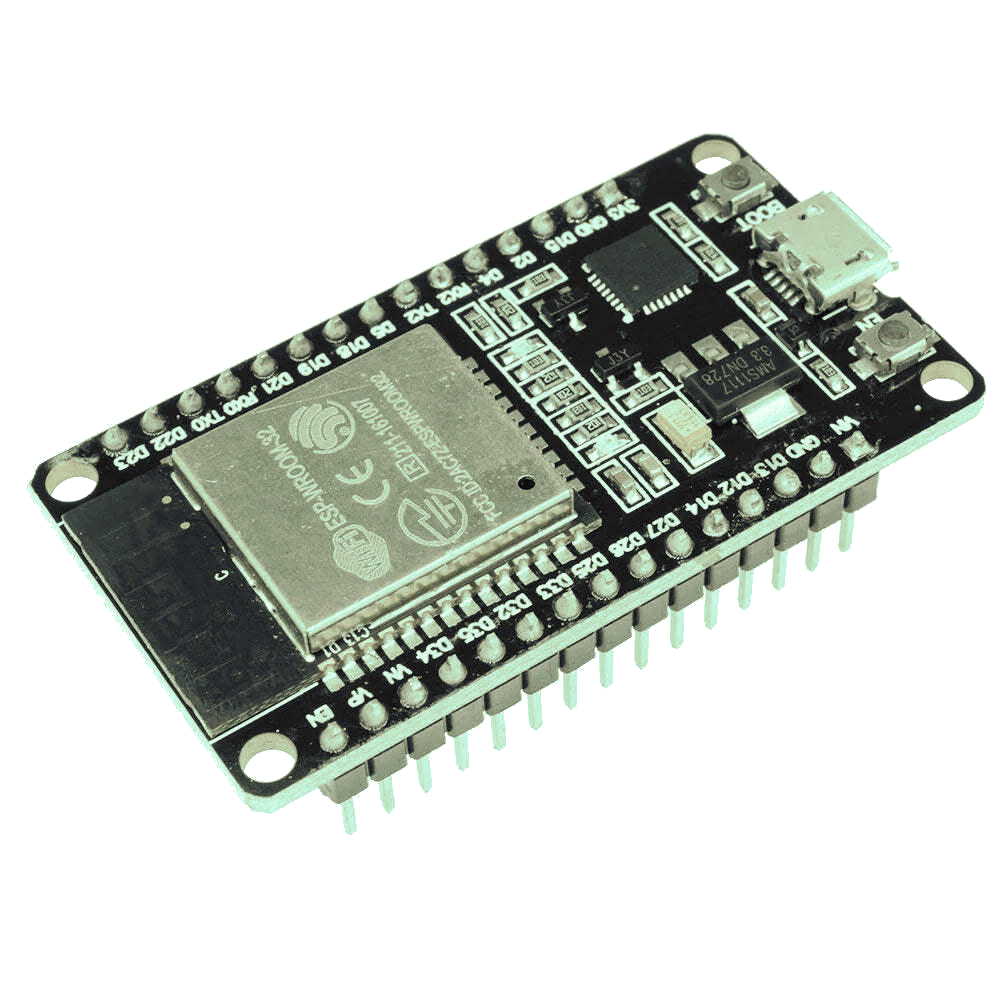
\includegraphics[height = 2cm]{pics/esp.png} & \multirow{2}{*}{4 MB} & \multirow{2}{*}{240 MHz} & \multirow{2}{*}{520 KB} \\
%                     ESP32 & 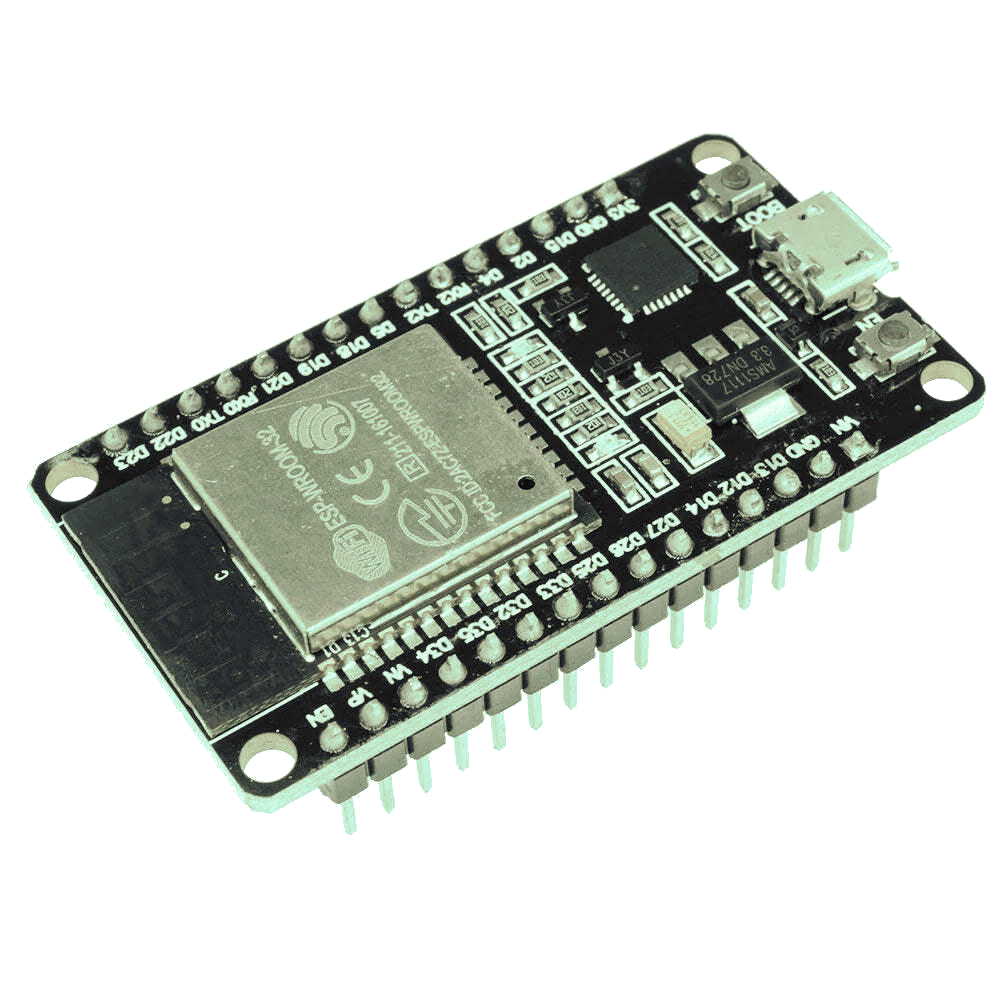
\includegraphics[height = 1.3cm]{pics/esp.png} & 4 MB & 240 MHz & 520 KB \\
%                     \midrule
%
%                     % 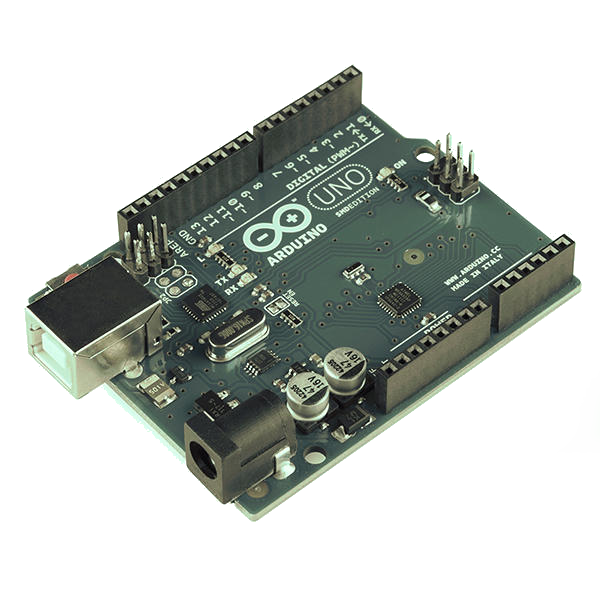
\includegraphics[height = 2cm]{pics/arduino.png} & \multirow{2}{*}{32 KB} & \multirow{2}{*}{16 MHz} & \multirow{2}{*}{2 KB} \\
%                     Arduino UNO & 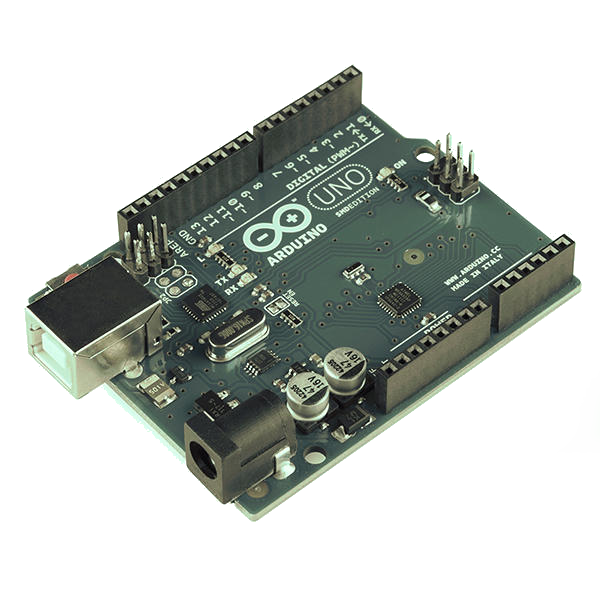
\includegraphics[height = 1.3cm]{pics/arduino.png} & 32 KB & 16 MHz & 2 KB \\
%                     \midrule
%
%                     % 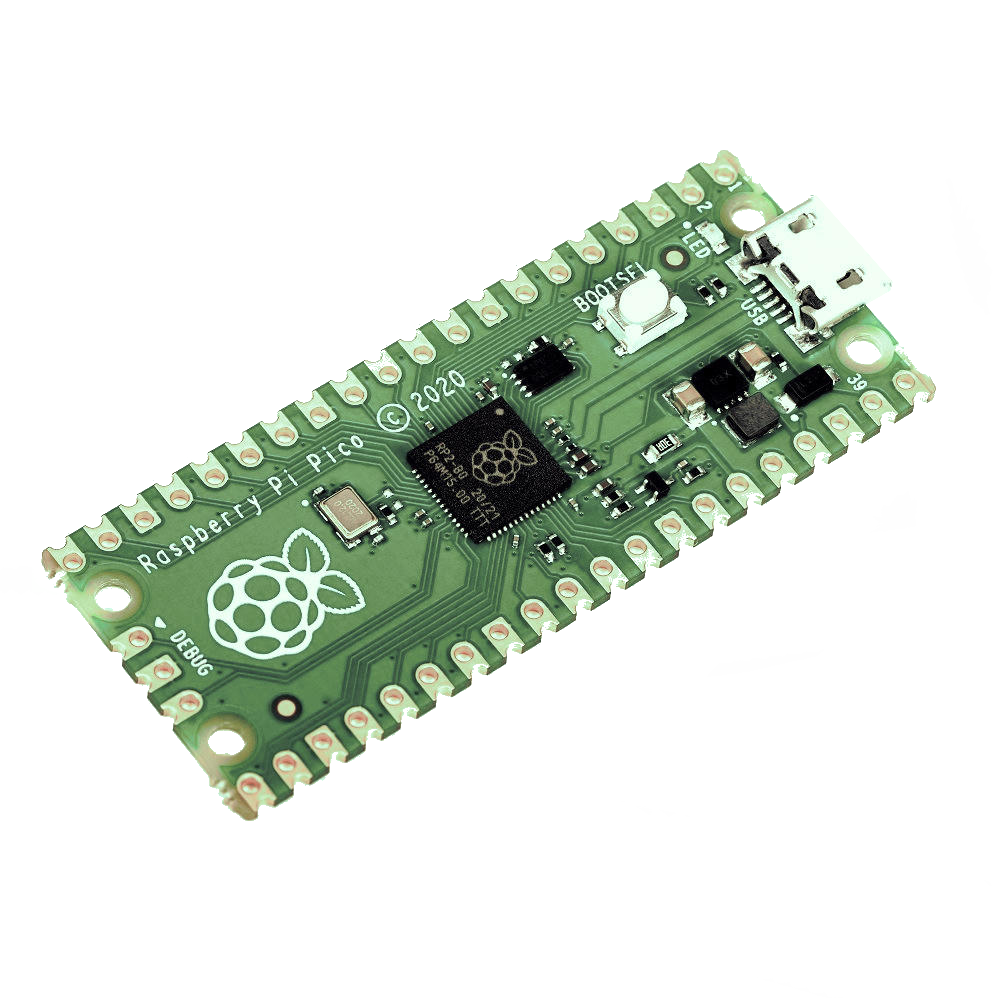
\includegraphics[height = 2cm]{pics/pico.png} & \multirow{2}{*}{2 MB} & \multirow{2}{*}{125 MHz} & \multirow{2}{*}{264 KB} \\
%                     Raspberry Pi Pico & 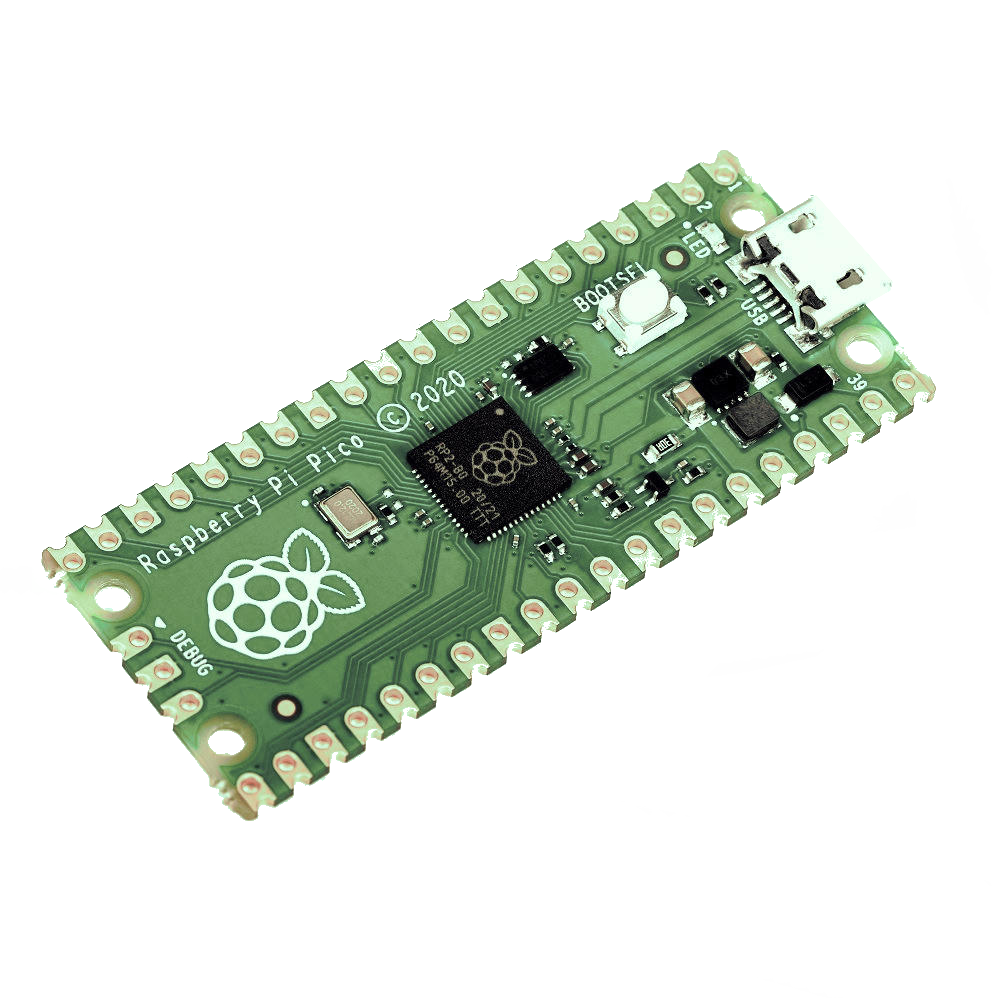
\includegraphics[height = 1.3cm]{pics/pico.png} & 2 MB & 125 MHz & 264 KB \\
%
%                     \bottomrule
%
%                 \end{tabularx}
%
%
%             \end{minipage}
%
%         }
%         ;
%
%     \end{tikzpicture}
%
% \end{frame}
%
% %% With Great Power Comes Great Responsibility
% \begin{frame} {}
%
%     \begin{tikzpicture} [
%             remember picture,
%             overlay,
%         ]
%
%         \tikzframetitleright{With Great Power} {Comes Great Responsibility}
%
%         \draw
%         ($(current page.south)!0.5!(current page.south |- frametitle.south)$)
%         coordinate (contentCenter)
%         (frametitle.east |- contentCenter)
%         ++(0, 0.5)
%         node [anchor = east] {
%             \begin{minipage} {0.575\textwidth}
%
%                 Just as TinyML has its advantages, it has its disadvantages.
%
%                 \begin{itemize}
%
%                     \item The ML model is \alert{compressed} using various techniques to fit into the
%                         \alert{constrains} of the microcontroller.
%
%                     \item The compressed ML model will be \alert{low fidelity} one.
%
%                     \item The low fidelity model \alert{may} or \alert{may not} be applicable for the
%                         given task.
%
%                     \item Sometimes we need \alert{cascade} different models having different fidelity.
%
%                 \end{itemize}
%
%             \end{minipage}
%         }
%         ;
%
%         \draw
%         ($(current page.center)!0.5!(current page.west)$) ++(-0.25, -4.95cm) coordinate (center)
%         ;
%
%         \def\stageGap{0.2}
%         \def\stageHeight{2.30}
%         \def\baseLen{8}
%         \def\stageDec{0.5}
%
%         \foreach \x in {7,6,5} {
%             \def\baseLen{\x}
%             \filldraw [
%                 rounded corners = 0.7cm,
%             ]
%             (center) ++(-\baseLen / 2, 0) coordinate (bl)
%             ++(\baseLen, 0) coordinate (br)
%             ++(-\stageDec, \stageHeight) coordinate (tr)
%             ++({(2 * \stageDec) - \baseLen}, 0) coordinate (tl)
%
%             (center) ++(0, \stageHeight / 2) coordinate (center-\x)
%             (bl) -- (br) -- (tr) -- (tl) -- cycle
%             ;
%             \draw
%             (center)
%             (center) ++(0, \stageHeight + \stageGap) coordinate (center)
%             ;
%
%         }
%
%         \node [white, anchor = center] at (center-7) {
%             \begin{minipage} {0.5\textwidth}
%                 \centering
%                 Low Fidelity ML Model \\
%                 (Always running.)
%             \end{minipage}
%         }
%         ;
%
%         \node [white, anchor = center] at (center-6) {
%             \begin{minipage} {0.5\textwidth}
%                 \centering
%                 Higher Fidelity ML Model \\
%                 (Triggered from below.)
%             \end{minipage}
%         }
%         ;
%
%         \node [white, anchor = center] at (center-5) {
%             \begin{minipage} {0.5\textwidth}
%                 \centering
%                 Main CPU \\
%                 (Triggered from below.)
%             \end{minipage}
%         }
%         ;
%
%         \def\baseLen{4}
%         \def\stageDec{1.5}
%
%         \filldraw [
%             rounded corners = 0.7cm,
%         ]
%         (center) ++(-\baseLen / 2, 0) coordinate (bl)
%         ++(\baseLen, 0) coordinate (br)
%         ++(\stageDec, \stageHeight) coordinate (tr)
%         ++({-(2 * \stageDec) - \baseLen}, 0) coordinate (tl)
%
%         (center) ++(0, \stageHeight / 2) coordinate (center-title)
%         (bl) -- (br) -- (tr) -- (tl) -- cycle
%         ;
%
%         \draw [white]
%         (center-title) node [anchor = center] {
%             \large Cascading ML Models
%         }
%         ;
%
%     \end{tikzpicture}
%
% \end{frame}
%
% %% The Essence of Tiny Machine Learning
% \begin{frame} {}
%     \begin{tikzpicture} [
%             remember picture,
%             overlay,
%         ]
%
%         \def\bgRomGap{0.3cm}
%         \def\bgRomOp{0.7}
%
%         % \begin{scope} [
%         %         transform canvas = {
%         %             xshift = 6.313cm,
%         %             yshift = -1.5cm,
%         %         },
%         %     ]
%         %     \filldraw [
%         %         ultra thick,
%         %         rotate = 45,
%         %         opacity = \bgRomOp,
%         %         colorLightGreen,
%         %         rounded corners = 0.7cm,
%         %     ]
%         %     (current page.west)
%         %     rectangle ++(-8cm, 8cm)
%         %     ;
%         %
%         %     \filldraw [
%         %         ultra thick,
%         %         rotate = 45,
%         %         opacity = \bgRomOp,
%         %         colorLightSageGreen,
%         %         rounded corners = 0.7cm,
%         %     ]
%         %     (current page.west) ++(\bgRomGap, 0) rectangle ++(2.5, 2.5)
%         %     ;
%         %
%         %     \filldraw [
%         %         ultra thick,
%         %         rotate = 45,
%         %         opacity = \bgRomOp,
%         %         colorLightGreen,
%         %         rounded corners = 0.7cm,
%         %     ]
%         %     (current page.west) ++(\bgRomGap, -\bgRomGap) rectangle ++(4, -4)
%         %     ;
%         %
%         %     \filldraw [
%         %         ultra thick,
%         %         rotate = 45,
%         %         opacity = \bgRomOp,
%         %         colorLightSageGreen,
%         %         rounded corners = 0.7cm,
%         %     ]
%         %     (current page.west) ++(0, -\bgRomGap) rectangle ++(-4, -4)
%         %     ;
%         %
%         %     \filldraw [
%         %         ultra thick,
%         %         rotate = 45,
%         %         opacity = \bgRomOp,
%         %         colorLightSageGreen,
%         %         rounded corners = 0.7cm,
%         %     ]
%         %     (current page.west) ++(0, -\bgRomGap - 4cm)  ++(\bgRomGap, -\bgRomGap) rectangle ++(10, -10)
%         %     ;
%         %
%         %
%         % \end{scope}
%         %
%         % \draw [thin, step = 0.1, white, opacity = 0.40]
%         % (current page.north west) grid (current page.south east)
%         % ;
%
%         \tikzframetitlelongright{The Essence of} {Running ML on Microcontrollers}
%
%         \draw
%         (current page.center |- frametitle.south)
%         node [anchor = north, below = 8pt] {
%             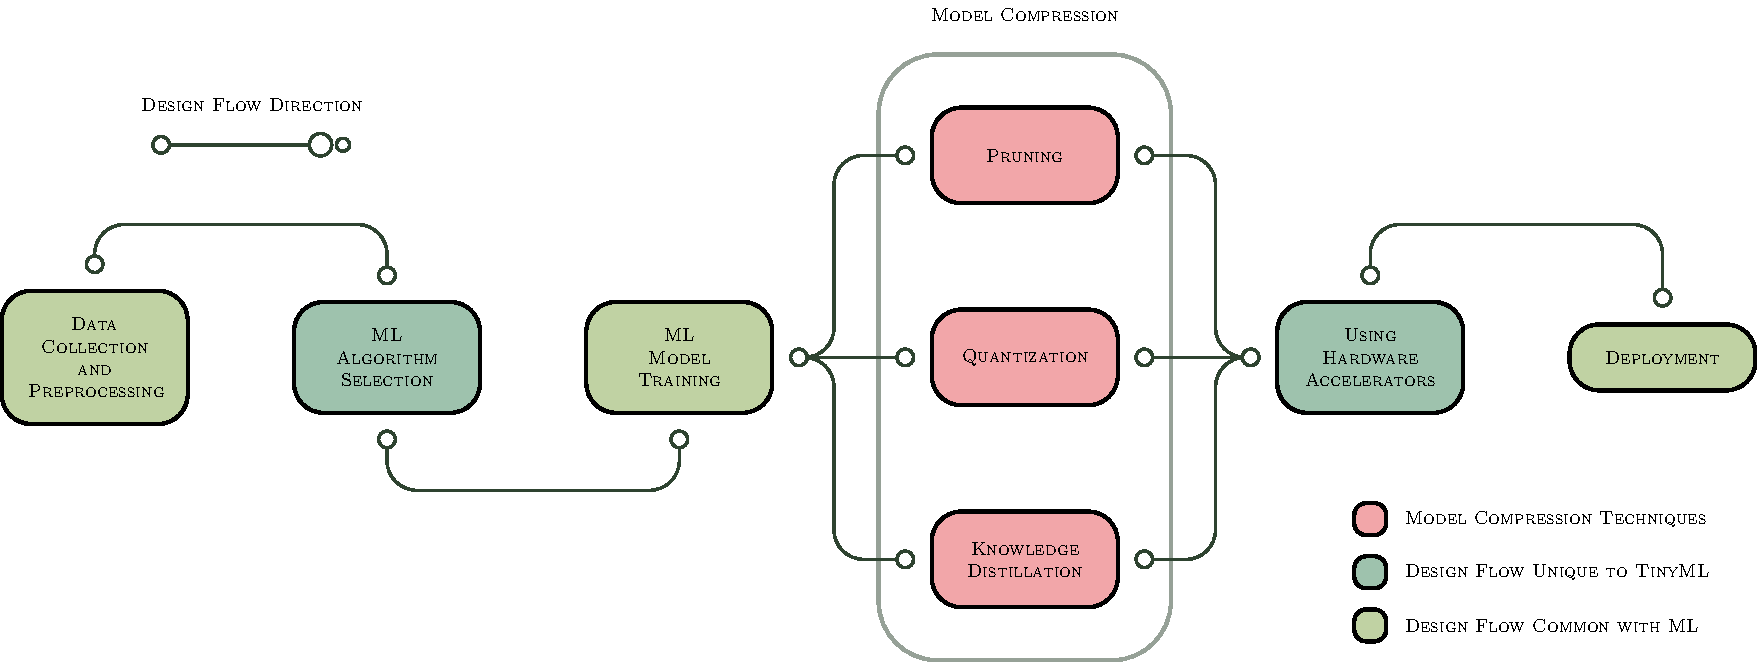
\includegraphics[width = 0.95\paperwidth]{tikzpics/endDesignFlow.pdf}
%         }
%         ;
%
%     \end{tikzpicture}
% \end{frame}
%
% %% Quantization: Shrinking the Parameters
% \begin{frame} {}
%
%     \begin{tikzpicture} [
%             remember picture,
%             overlay,
%         ]
%
%         \tikzframetitleleft{Quantization:} {Shrinking the Parameters}
%
%         % \draw
%         % (current page.center) ++(0, -1)
%         % node [anchor = center] {
%         %     \includegraphics[width = 0.9\paperwidth]{pics/qp.pdf}
%         % }
%         % ;
%
%         \draw
%         (current page.center) ++(0, -1)
%         node [anchor = center] {
%             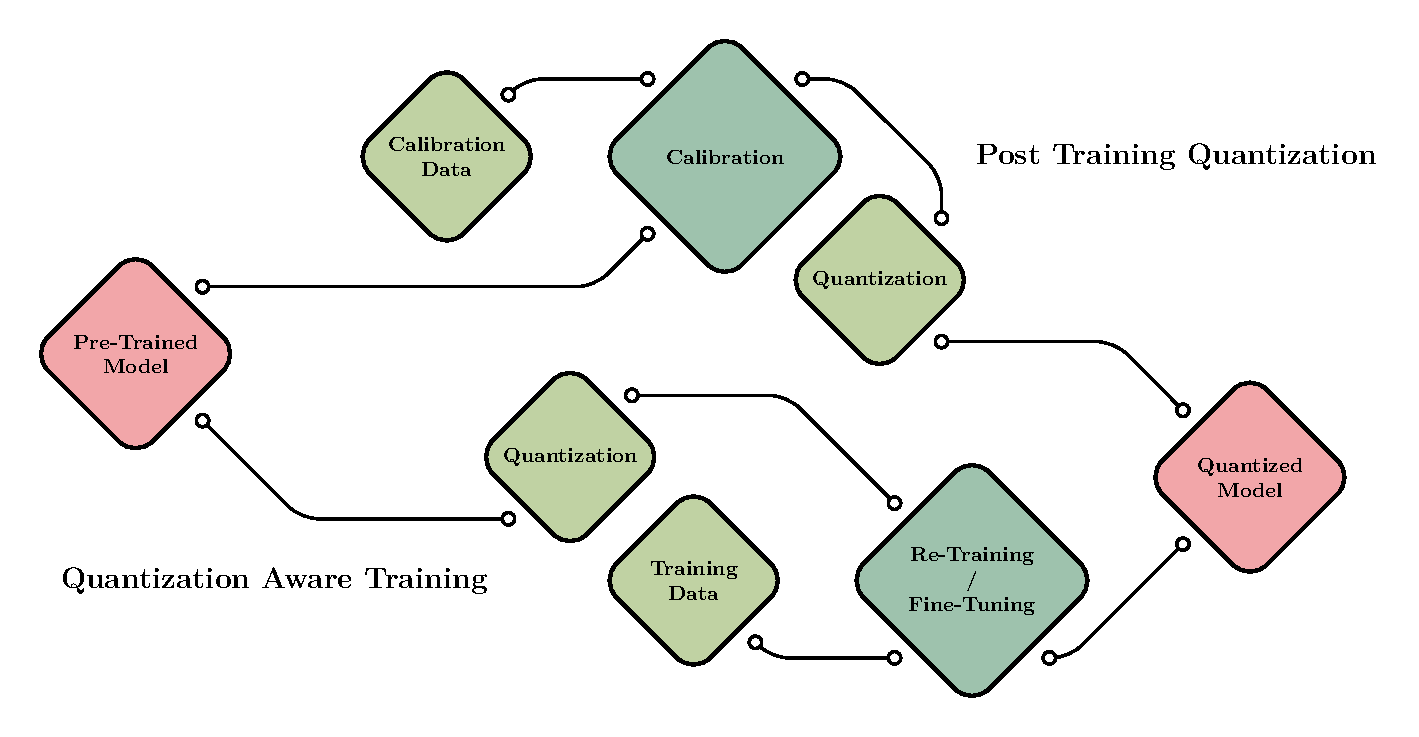
\includegraphics[height = 0.8\paperheight]{tikzpics/endQuantization.pdf}
%         }
%         ;
%
%     \end{tikzpicture}
%
% \end{frame}
%
% %% Pruning: Cutting Down Connections
% \begin{frame} {}
%
%     \begin{tikzpicture} [
%             remember picture,
%             overlay,
%         ]
%
%         \tikzframetitlelongleft{Pruning:} {Cutting Down Connections}
%
%         \draw
%         (current page.center) ++(0, -1)
%         node [anchor = center] {
%             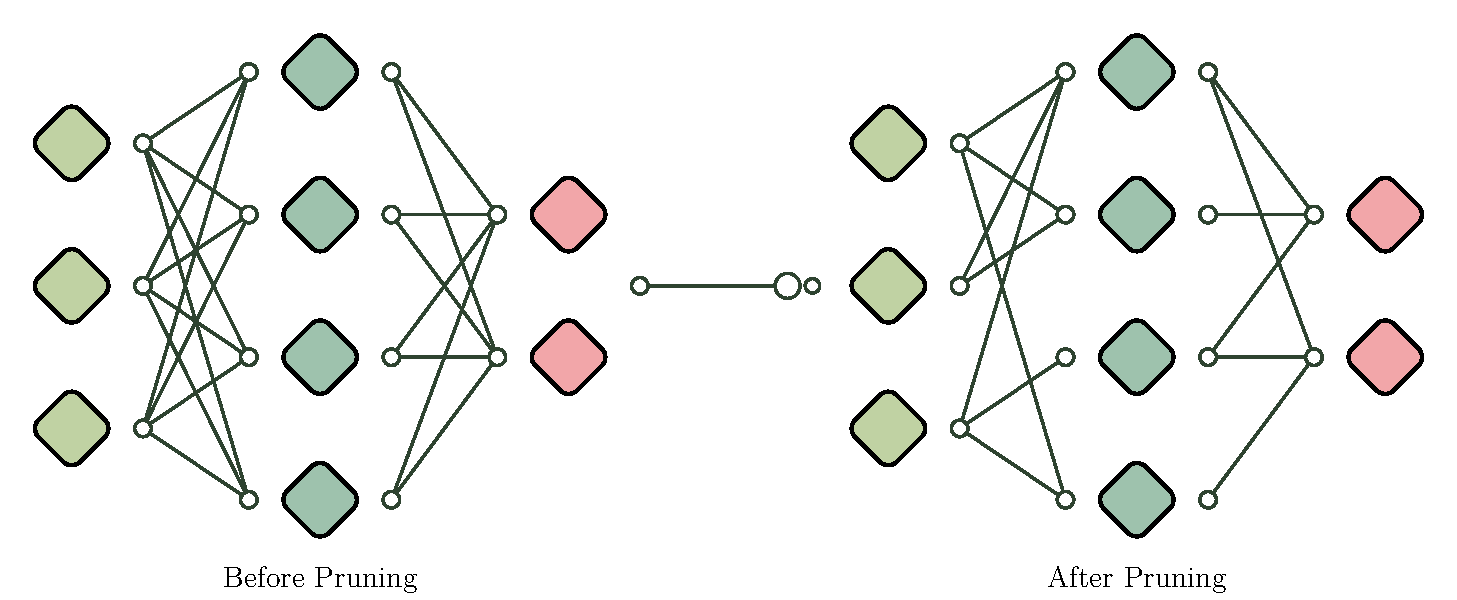
\includegraphics[width = 0.9\paperwidth]{tikzpics/endPruning.pdf}
%         }
%         ;
%
%     \end{tikzpicture}
%
% \end{frame}
%
% %% Knowledge Distillation: Teacher and Student Learning
% \begin{frame} {}
%
%     \begin{tikzpicture} [
%             remember picture,
%             overlay,
%         ]
%
%         \tikzframetitlelongright{Knowledge Distillation:} {Teacher and Student Learning}
%
%         \draw
%         (current page.center) ++(0, -1)
%         node [anchor = center] {
%             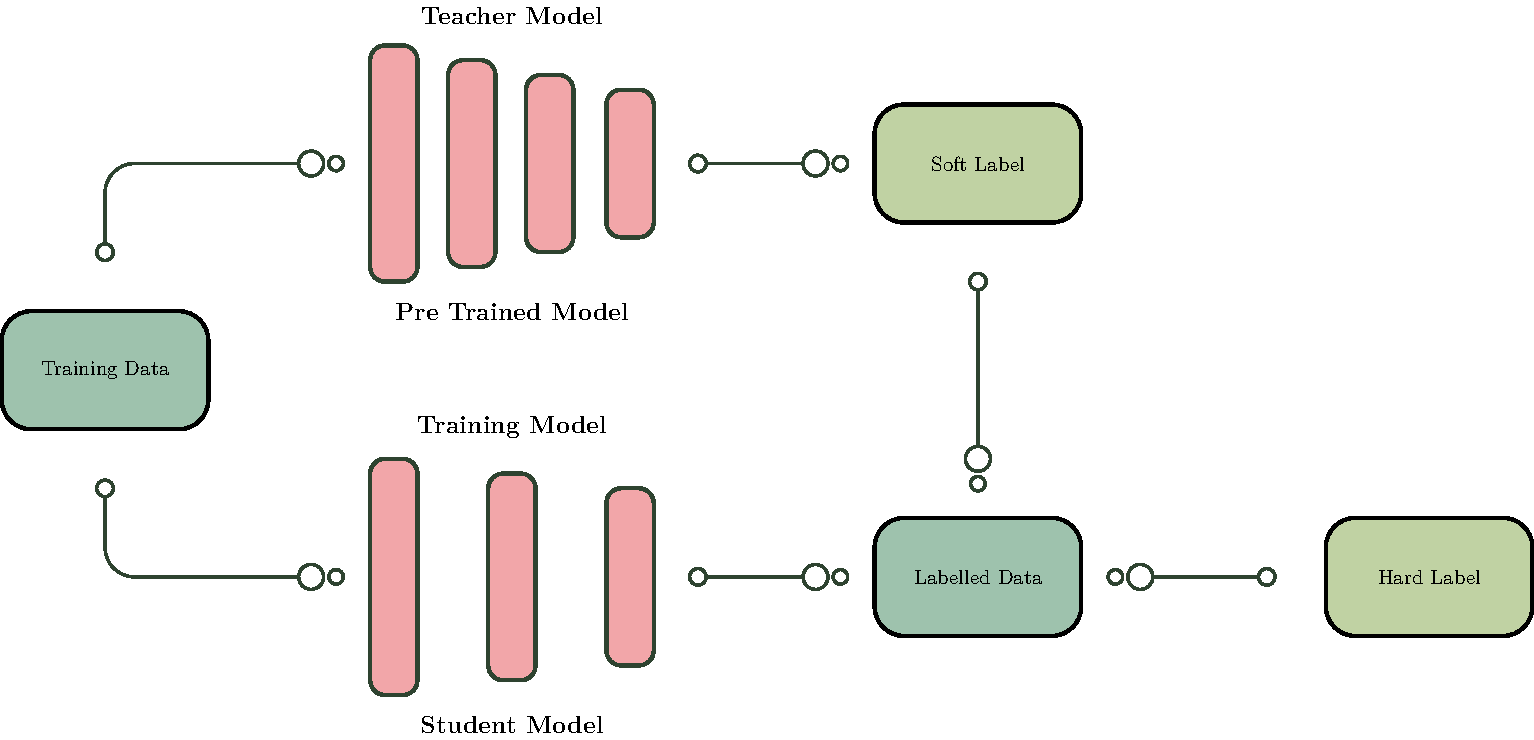
\includegraphics[width = 0.85\paperwidth]{tikzpics/endKnowledgeDistillation.pdf}
%         }
%         ;
%
%     \end{tikzpicture}
%
% \end{frame}
%
% %% Software: Frameworks and Tool Chains
% \begin{frame} {}
%
%     \begin{tikzpicture} [
%             remember picture,
%             overlay,
%         ]
%
%         \tikzframetitlelongright{Software:} {Frameworks and Tool Chains}
%
%         \filldraw
%
%         ($(current page.west)!0.20!(current page.east)$) coordinate (v1)
%         ($(current page.west)!0.5!(current page.east)$) coordinate (v2)
%         ($(current page.west)!0.80!(current page.east)$) coordinate (v3)
%
%         (current page.north) ++(0, -1.5) coordinate (top)
%
%         ($(top)!0.33!(current page.south)$) coordinate (h1)
%         ($(top)!0.66!(current page.south)$) coordinate (h2)
%
%         (v1 |- h1) ++(-0.5, 0) coordinate (tflPic)
%
%         (v3 |- h2) ++(0.5, -0.5) coordinate (eiPic)
%
%         (tflPic) circle (0.2cm)
%         (eiPic) circle (0.2cm)
%         ;
%
%         \def\picSide{3cm}
%
%
%         \begin{scope}
%             \clip [
%                 rounded corners = 0.4cm,
%             ]
%             (tflPic) ++(-\picSide / 2, -\picSide / 2) rectangle ++(\picSide, \picSide)
%             ;
%
%             \draw
%             (tflPic)
%             node (tflPic) [
%                 anchor = center,
%             ] {
%                 
\includegraphics[width = \picSide] {pics/tfl.png}
%             }
%             ;
%
%         \end{scope}
%
%         \begin{scope}
%             \filldraw [
%                 colorDarkGreen,
%                 rounded corners = 0.4cm,
%             ]
%             (eiPic) ++(-\picSide / 2, -\picSide / 2) rectangle ++(\picSide, \picSide)
%             ;
%
%             \draw
%             (eiPic)
%             node (eiPic) [
%                 anchor = center,
%             ] {
%                 
\includegraphics[width = \picSide] {pics/ei.png}
%             }
%             ;
%
%         \end{scope}
%
%         \draw
%         (tflPic.north east) ++(0, -0.25)
%         node (tflTitle) [anchor = north west] {
%             \begin{minipage} {0.75\textwidth}
%                 {\large {TensorFlow Lite}}
%             \end{minipage}
%         }
%         ;
%
%         \draw
%         (eiPic.north west) ++(0, -0.25)
%         node (eiTitle) [anchor = north east] {
%             \begin{minipage} {0.75\textwidth}
%                 \raggedleft
%                 {\large {Edge Impulse}}
%             \end{minipage}
%         }
%         ;
%
%
%         \draw
%         ($(tflTitle.south west)!0.5!(tflTitle.south west |- tflPic.south)$)
%         node [anchor = west] {
%             \begin{minipage} {0.75\textwidth}
%                 \begin{itemize}
%                     \item Developed by \alert{Google} building and deploying ML Models on Embedded Systems.
%                     \item Open-source Framework.
%                     \item Gives more control.
%                 \end{itemize}
%             \end{minipage}
%         }
%         ;
%
%         \draw
%         ($(eiTitle.south east)!0.5!(eiTitle.south east |- eiPic.south)$)
%         node [anchor = east] {
%             \begin{minipage} {0.75\textwidth}
%                 \begin{itemize}
%                     \item Offers a comprehensive set of tools for the entire embedded machine learning lifecycle.
%                     \item \alert{Simplifies} the process of building edge AI solutions.
%                 \end{itemize}
%             \end{minipage}
%         }
%         ;
%
%     \end{tikzpicture}
%
% \end{frame}
%
% %% General Application of TinyML
% \begin{frame} {}
%
%     \begin{tikzpicture} [
%             remember picture,
%             overlay,
%         ]
%
%         \tikzframetitleleft {General} {Applications of TinyML}
%
%         \filldraw
%         ($(current page.center)!0.5!(current page.west)$) ++(1.5cm, -3.0cm) coordinate (center)
%         ;
%
%         \subSquare{s1}{center}{padBotCorner} % second
%         \subSquare{s2}{center}{padLeftCorner} % third
%         \subSquare{s3}{center}{padRightCorner} % first
%         \subSquare{s4}{s2-padRightCorner}{padBotCorner} % fourth
%
%         \subSquare{s5}{s4-padBotCorner}{padLeftCorner} % fifth
%
%         \subSquare{s6}{s4-padRightCorner}{padBotCorner} % sixth
%
%         \subSquare{tmpS1}{s1-padBotCorner}{padTopCorner} % fourth
%         \subSquare{tmpS2}{s4-padBotCorner}{padTopCorner} % fourth
%         \subSquare{tmpS3}{s4-padRightCorner}{padLeftCorner} % fourth
%
%         \drawSubSquare{colorLightGreen,}{s1}
%         \drawSubSquare{colorLightSageGreen,}{s2}
%         \drawSubSquare{colorLightSageGreen,}{s3}
%         \drawSubSquare{colorLightGreen,}{s4}
%
%         \drawSubSquare{colorLightSageGreen,}{s5}
%         \drawSubSquare{colorLightSageGreen,}{s6}
%
%         \drawSubSquare{colorLightGreen,}{tmpS1}
%         \drawSubSquare{colorLightGreen,}{tmpS2}
%         \drawSubSquare{colorLightGreen,}{tmpS3}
%
%         \node [anchor = center] at (s1-center) {
%             \begin{minipage} {\squareSide}
%                 \centering
%                 \large Agriculture \\ Smart Farming
%             \end{minipage}
%         }
%         ;
%
%         \node [anchor = center] at (s3-center) {
%             \begin{minipage} {\squareSide}
%                 \centering
%                 \large Industrial \\ Predictive Maintenance
%             \end{minipage}
%         }
%         ;
%
%         \node [anchor = center] at (s2-center) {
%             \begin{minipage} {\squareSide}
%                 \centering
%                 \large Smart Homes \\ Gesture and Voice Control
%             \end{minipage}
%         }
%         ;
%
%         \node [anchor = center] at (s4-center) {
%             \begin{minipage} {\squareSide}
%                 \centering
%                 \large Healthcare \\ Smart Wearables
%             \end{minipage}
%         }
%         ;
%
%         \node [anchor = center] at (s5-center) {
%             \begin{minipage} {\squareSide}
%                 \centering
%                 \large Automated \\ Speech Recognition
%             \end{minipage}
%         }
%         ;
%
%         \node [anchor = center] at (s6-center) {
%             \begin{minipage} {\squareSide}
%                 \centering
%                 \large Wildlife \\ Conservation in Remote Areas
%             \end{minipage}
%         }
%         ;
%
%     \end{tikzpicture}
%
% \end{frame}
%
% %% Applications of TinyML in Agriculture
% \begin{frame} {}
%
%     \begin{tikzpicture} [
%             remember picture,
%             overlay,
%         ]
%
%         \tikzframetitleleft{Applications of} {TinyML in Agriculture}
%
%         \filldraw
%
%         (current page.west) ++(1, 0) coordinate (west)
%         (current page.east) ++(-1, 0) coordinate (east)
%
%         ($(west)!0.15!(east)$) coordinate (v1)
%         ($(west)!0.5!(east)$) coordinate (v2)
%         ($(west)!0.85!(east)$) coordinate (v3)
%         % ($(west)!0.875!(east)$) coordinate (v4)
%
%         % ($(west)!0.125!(east)$) coordinate (v1)
%         % ($(west)!0.375!(east)$) coordinate (v2)
%         % ($(west)!0.625!(east)$) coordinate (v3)
%         % ($(west)!0.875!(east)$) coordinate (v4)
%
%         (current page.north) ++(0, -2.5) coordinate (top)
%
%         ($(top)!0.33!(current page.south)$) coordinate (h1)
%         ($(top)!0.66!(current page.south)$) coordinate (h2)
%
%         (v1 |- h1) coordinate (p1)
%         (v2 |- h1) coordinate (p2)
%         (v3 |- h1) coordinate (p3)
%
%         ;
%
%         \subPicSquare {s1} {p1} {center}
%         \putPicInRombus {} {} {s1} {pics/leaves.png}
%
%         \subPicSquare {s2} {p2} {center}
%         \putPicInRombus {} {} {s2} {pics/greenhouse.png}
%
%         \subPicSquare {s3} {p3} {center}
%         \putPicInRombus {} {++(0.25,0)} {s3} {pics/apples.png}
%
%         \draw (s1-padBotCorner) node [anchor = north, below = -4pt] {
%             \begin{minipage} {\picSquareDiagonal}
%                 \centering
%                 Plant Disease \\ Detection %% will stay
%             \end{minipage}
%         } ;
%         \draw (s3-padBotCorner) node [anchor = north, below = -4pt] {
%             \begin{minipage} {\picSquareDiagonal}
%                 \centering
%                 Fruit Detection \\ In Plants
%             \end{minipage}
%         } ;
%
%         \draw (s2-padBotCorner) node [anchor = north, below = -4pt] {
%             \begin{minipage} {\picSquareDiagonal}
%                 \centering
%                 Micro Climate \\ Management
%             \end{minipage}
%         } ;
%
%     \end{tikzpicture}
%
% \end{frame}

%% Case Study: Plant Disease Detection
\begin{frame} {}

    \begin{tikzpicture} [
            remember picture,
            overlay,
        ]

        \tikzframetitleright{Case Study:} {Plant Disease Detection}

        \draw
        (current page.north west) ++(1, -1) coordinate (csPic)
        ;

        \subCsPicSquare {csPic} {csPic} {topLeftCorner}

        \putCsPicInSquare {} {} {csPic} {width = \csPicSquareSide,} {pics/disease_detection.png}

        \draw [
            very thick,
            colorLightSageGreen,
            line cap = round,
        ]

        (csPic-botLeftCorner |- csPic-pBot) ++(0, -0.1cm) coordinate (lineStart)
        (lineStart -| current page.east) ++(-1, 0) coordinate (lineEnd)

        (lineStart) -- (lineEnd)

        ;

        \draw
        (frametitle.south -| csPic-pRight) ++(0, -0.3)
        node [anchor = north west] {
            \begin{minipage} {9.85cm}
                \begin{itemize}
                    \item Developed a TinyML system to detect \alert{Brown Streak} and \alert{Mosaic} Disease on Cassava plants.
                    \item Held an comparative study on \alert{TinyML} based system vs \alert{Cloud} based system.
                    \item For farmers in the remote places of \alert{Ghana} (West Africa).
                \end{itemize}
            \end{minipage}
        }
        ;

        \draw
        (csPic-botLeftCorner |- csPic-pBot) ++(0, -\csPicSquareGap - 0.2cm) coordinate (bcTop)
        (current page.south) ++(0, 1) coordinate (bcBot)
        (bcTop -| bcBot)
        node [
            anchor = north,
            fill = colorLightSageGreen,
            inner sep = 0.25cm,
            rounded corners = 0.5cm,
            minimum width = 13.85cm,
            minimum height = 2.7cm,
        ] {
            \begin{minipage} {0.925\textwidth}
                \vspace{0.25cm}
                % \begin{itemize}
                %     \item This is interesting. This is interesting. This is interesting. This is interesting.
                %     \item This is interesting. This is interesting. This is interesting. This is interesting.
                %     \item This is interesting. This is interesting. This is interesting. This is interesting.
                % \end{itemize}
                \vspace{0.25cm}
            \end{minipage}
        }
        ;


    \end{tikzpicture}

\end{frame}

\end{document}
